\documentclass[11pt,a4paper]{article}

% ── Packages ──────────────────────────────────────────────
\usepackage[utf8]{inputenc}
\usepackage[T1]{fontenc}
\usepackage[margin=1in]{geometry}
\usepackage{hyperref}
\usepackage{xcolor}
\usepackage{listings}
\usepackage{booktabs}
\usepackage{longtable}
\usepackage{array}
\usepackage{amsmath,amssymb}
\usepackage{enumitem}
\usepackage{fancyhdr}
\usepackage{titlesec}
\usepackage{caption}
\usepackage{subcaption}
\usepackage{mdframed}
\usepackage{natbib}
\usepackage{multirow}
\usepackage{graphicx}

% ── Colors & Hyperref ─────────────────────────────────────
\definecolor{codebackground}{HTML}{F5F5F5}
\definecolor{codekeyword}{HTML}{0000FF}
\definecolor{codecomment}{HTML}{228B22}
\definecolor{linkcolor}{HTML}{2563EB}

\hypersetup{
    colorlinks=true,
    linkcolor=linkcolor,
    urlcolor=linkcolor,
    citecolor=linkcolor,
    pdftitle={Dynamic Token Merging for Encoder-Only Transformers},
}

% ── Code listing style ────────────────────────────────────
\lstdefinestyle{codestyle}{
    backgroundcolor=\color{codebackground},
    basicstyle=\ttfamily\small,
    keywordstyle=\color{codekeyword}\bfseries,
    commentstyle=\color{codecomment}\itshape,
    breaklines=true,
    keepspaces=true,
    frame=single,
    framerule=0.4pt,
    rulecolor=\color{black!20},
    xleftmargin=1em,
    xrightmargin=0.5em,
    aboveskip=0.8em,
    belowskip=0.6em,
}
\lstset{style=codestyle}

% ── Header/Footer ─────────────────────────────────────────
\pagestyle{fancy}
\fancyhf{}
\fancyhead[L]{\small\leftmark}
\fancyhead[R]{\small CS224N Final Project Report}
\fancyfoot[C]{\thepage}
\renewcommand{\headrulewidth}{0.4pt}

% ── Column types ──────────────────────────────────────────
\newcolumntype{L}[1]{>{\raggedright\arraybackslash}p{#1}}
\newcolumntype{C}[1]{>{\centering\arraybackslash}p{#1}}

% ── Figure paths ──────────────────────────────────────────
\graphicspath{{figures/}}

% ══════════════════════════════════════════════════════════
\begin{document}

% ── Title ─────────────────────────────────────────────────
\begin{center}
    {\LARGE \textbf{Dynamic Token Merging for Encoder-Only Transformers:\\[0.3em]
    Adapting MrT5's Delete Gate to BERT and XLM-RoBERTa}}\\[1.5em]
    {\large \textbf{CS224N: Natural Language Processing with Deep Learning --- Final Project Report}}\\[1em]
    Hiva Zaad \quad \texttt{hiva@stanford.edu}\\[0.5em]
    Alina Tianhui Huang \quad \texttt{alinah@stanford.edu}\\[0.5em]
    Aronima Dass \quad \texttt{adass@stanford.edu}\\[0.5em]
    \textbf{Mentor: Julie Kallini} \quad \emph{kallini@stanford.edu}\\[0.3em]
    \textbf{Sharing:} This report may be posted on the CS224N website.
\end{center}

\bigskip

% ══════════════════════════════════════════════════════════
\begin{abstract}
Transformer-based language models apply uniform computation to every input token, regardless of token informativeness.
The MrT5 paper \citep{kallini2024mrt5} introduced a \emph{Dynamic Token Merging} (DTM) delete gate for byte-level encoder-decoder models, achieving up to 60\% sequence length reduction with minimal perplexity degradation.
We ask: does this mechanism generalise to subword-based encoder-only architectures used for discriminative NLU?
We implement \textbf{MrBERT} and \textbf{MrXLMR}, adapting the MrT5 delete gate to BERT-base and XLM-RoBERTa-base respectively.
Our gate fires after encoder layer~3 (out of~12), uses a PI controller to hit a target deletion rate~$\delta$, and introduces a novel \emph{pre-deletion blending} mechanism that makes extractive QA viable under token deletion.
Evaluated across six tasks --- SNLI, SQuAD, SST-2, MRPC, IMDB, and TyDi~QA --- our results show:
MrBERT at 30\% deletion achieves \textbf{90.21\%} SNLI accuracy (only 0.27pp below baseline) at \textbf{1.89$\times$} A100 inference speedup;
SST-2 drops by only 0.62pp (97.29\%$\to$96.67\%), while MRPC shows a larger 17.32pp drop, revealing dataset-specific sensitivity;
TyDi~QA span EM recovers from 0.10 (no blending) to 0.35 (layer~9 + blending), matching BERT end accuracy.
A random-deletion baseline scores 2.95pp below MrBERT-30\% on SNLI, confirming learned token selection.
MrXLMR achieves 82.27\% on SNLI at 30\% deletion (baseline 89.85\%), suggesting XLM-R requires careful tuning for high deletion rates.
\end{abstract}


% ══════════════════════════════════════════════════════════
\section{Introduction}
\label{sec:introduction}

Large pretrained transformers such as BERT \citep{devlin2019bert} and XLM-RoBERTa \citep{conneau2020xlmr} achieve state-of-the-art performance across a wide range of NLU tasks. However, their computational cost scales quadratically with sequence length due to self-attention, making inference expensive. A natural question is whether all tokens are equally important for a given task: for a sentiment classification example, function words like ``the'' and ``of'' carry little discriminative content, while content words like ``terrible'' or ``outstanding'' are crucial.

The MrT5 paper \citep{kallini2024mrt5} proposes \emph{Dynamic Token Merging} (DTM): a learned scalar gate inserted after an early encoder layer that assigns each token a deletion score. Low-scoring tokens are masked out of subsequent attention computations (soft deletion) or physically removed (hard deletion). MrT5 demonstrates this on a byte-level T5 model, showing up to 60\% sequence reduction at minimal perplexity cost.

We address the open question: \textbf{does this mechanism transfer to subword-based encoder-only models trained on discriminative NLU tasks?} The transfer is non-trivial because:

\begin{enumerate}[nosep]
    \item BERT and XLM-R use subword tokenisation, not byte-level tokens, so token granularity and importance distributions differ.
    \item Encoder-only models pool to a single \texttt{[CLS]} vector for classification, creating a different information-flow bottleneck than encoder-decoder models.
    \item Extractive QA requires localising answer spans: answer tokens must survive deletion --- a hard constraint absent in language modelling.
    \item XLM-R spans 100 languages with a shared 250K SentencePiece vocabulary; importance patterns must generalise across scripts.
\end{enumerate}

Our contributions are:
\begin{itemize}[nosep]
    \item \textbf{MrBERT}: BERT-base with a MrT5-style delete gate, evaluated on SNLI, SST-2, MRPC, IMDB, SQuAD, and TyDi~QA.
    \item \textbf{MrXLMR}: XLM-RoBERTa-base with the same mechanism, evaluated on SNLI.
    \item \textbf{Pre-deletion blending}: a novel mechanism enabling extractive QA under deletion; span EM improves 3.5$\times$.
    \item \textbf{Comprehensive ablations}: PI controller necessity, gate layer placement (layers 1/3/6/9), soft vs.\ hard deletion gap, and deletion pattern analysis.
\end{itemize}


% ══════════════════════════════════════════════════════════
\section{Related Work}
\label{sec:related-work}

\textbf{MrT5} \citep{kallini2024mrt5}. The direct antecedent of this work. MrT5 attaches a scalar delete gate after a selected encoder layer of a T5-based byte-level model. A PI controller adjusts the deletion loss coefficient~$\alpha$ to track a target deletion rate. The gate adds fewer than 3K parameters to a 250M parameter model, achieving 50--60\% sequence reduction on language modelling tasks with minimal degradation.

\textbf{Efficient transformers.} Sparse attention methods (Longformer, BigBird) reduce attention from $O(n^2)$ to $O(n)$. Early-exit approaches (DeeBERT, PABEE) skip later layers for easy examples. Token pruning methods (TR-BERT, SpAtten, LTP) learn to drop tokens. Unlike these, our method is trained end-to-end with differentiable soft deletion and requires no architectural changes beyond the gate module.

\textbf{Token importance in BERT.} \citet{michel2019heads} and \citet{voita2019heads} showed many BERT attention heads are redundant. \citet{clark2019attention} found BERT attention aligns with syntactic structure; function words receive less attention in higher layers, consistent with our gate's deletion patterns (Section~\ref{sec:deletion-patterns}).


% ══════════════════════════════════════════════════════════
\section{Approach}
\label{sec:approach}

\subsection{Architecture Overview}

MrBERT is a pretrained BERT-base encoder with a lightweight delete gate inserted after a selected layer. The gate uses hidden states from that layer to compute a scalar score per token; the score is then used to mask tokens in all subsequent layers.

\begin{lstlisting}
Input tokens
     |
[Embeddings]
     |
Encoder layers 0-2   <- Full sequence (128 tokens)
     |
Encoder layer 3      <- Gate fires here
  [Delete Gate]
  LayerNorm -> Linear(768->1) -> ScaledSigmoid(-30)
     | gate values g in (-30, 0)
Soft/Hard deletion
     |
Encoder layers 4-11  <- Reduced sequence (~89 tokens at delta=0.3)
     |
Task head (CLS pooling -> classifier / span logits)
\end{lstlisting}

\textbf{BERT-base} \citep{devlin2019bert}: 12 layers, $d_{\text{model}}=768$, 12 heads, 110M parameters, WordPiece 30K vocabulary. \textbf{XLM-RoBERTa-base} \citep{conneau2020xlmr}: same dimensions, 277M parameters, SentencePiece 250K vocabulary.


\subsection{Delete Gate}
\label{sec:delete-gate}

The gate module (\texttt{SigmoidDeleteGate}) has three components:

\textbf{(1) LayerNorm.} The hidden state $\mathbf{h}_i$ from layer \texttt{delete\_gate\_layer} is normalised before projection, stabilising training.

\textbf{(2) Linear projection.} $z_i = \mathbf{W}\mathbf{h}_i + b$, with $\mathbf{W}\sim\mathcal{N}(0,0.02)$ and $b=10.0$. The large positive bias initialises the gate near zero deletion ($g\approx-0.001$), so the model starts from the pretrained baseline.

\textbf{(3) Scaled sigmoid.}
\begin{equation}
    g_i = s \cdot \sigma(-z_i), \qquad s = -30
    \label{eq:scaled-sigmoid}
\end{equation}
Gate values lie in $(-30,0)$: near~$0$ means keep, near~$-30$ means delete. Deletion threshold $\tau = s/2 = -15$. The gate adds only 2,305 parameters ($768+1$ weights $+$ $2{\times}768$ LayerNorm). \texttt{[CLS]}/\texttt{[SEP]} are always kept; \texttt{[PAD]} is always deleted.


\subsection{Soft and Hard Deletion}

During training, \textbf{soft deletion} adds $g_i$ as an attention bias:
\begin{equation}
    \tilde{a}(q, k_i) = a(q, k_i) + g_i
\end{equation}
Deleted tokens ($g_i\approx-30$) contribute negligible attention weight, while remaining differentiable for end-to-end training. We additionally apply softmax1 \citep{kallini2024mrt5}: replacing $\sum\exp(a_j)$ with $\sum\exp(a_j)+\exp(-\max_j a_j)$, allowing attention weights to sum to less than~1.

At inference, \textbf{hard deletion} physically removes positions where $g_i<\tau$, achieving real memory and compute savings.


\subsection{Pre-Deletion Blending}
\label{sec:pre-deletion-blending}

For extractive QA, deleted answer tokens produce corrupted representations at the task head. We introduce \textbf{pre-deletion blending}: for each token~$i$, blend weight $w_i = \text{clamp}(-g_i/30,0,1)$, and:
\begin{equation}
    \tilde{\mathbf{h}}_i = (1-w_i)\cdot\mathbf{h}_i^{(L)} + w_i\cdot\mathbf{h}_i^{(\text{gate})}
    \label{eq:blending}
\end{equation}
where $\mathbf{h}_i^{(L)}$ is the layer-11 output and $\mathbf{h}_i^{(\text{gate})}$ is the pre-gate hidden state. For kept tokens ($w_i\approx0$), the representation is unchanged. For deleted tokens ($w_i\approx1$), it falls back to the richer pre-gate representation. This also provides a gradient signal through deleted positions, preventing gate collapse during QA training (Section~\ref{sec:results-tydiqa}).


\subsection{PI Controller}
\label{sec:pi-controller}

A PI controller dynamically adjusts the deletion loss coefficient $\alpha$ to track target deletion rate $\delta$:
\begin{align}
    e_t &= \delta - r_t, \quad
    p_t = \gamma p_{t-1} + (1-\gamma)k_p e_t, \quad
    i_t = i_{t-1} + k_i e_t, \quad
    \alpha_t = \max(0, p_t+i_t)
\end{align}
Total loss: $\mathcal{L} = \mathcal{L}_{\text{task}} + \alpha_t\cdot\mathcal{L}_{\text{deletion}}$, where $\mathcal{L}_{\text{deletion}} = \text{mean}(g_i)$ over non-padding tokens. Parameters: $k_p=0.01$, $k_i=10^{-5}$, $\gamma=0.9$.


\subsection{Key Differences from MrT5}

\begin{table}[h]
\centering\small
\begin{tabular}{@{}lll@{}}
\toprule
\textbf{Aspect} & \textbf{MrT5} & \textbf{MrBERT / MrXLMR} \\
\midrule
Architecture       & Encoder-decoder (T5)    & Encoder-only \\
Tokenisation       & Byte-level (256 vocab)  & WordPiece 30K / SentencePiece 250K \\
Gate fires         & Before self-attention   & After full encoder layer (attn $+$ FFN) \\
Pre-deletion blend & None                    & Yes --- critical for QA \\
Gate init (bias)   & Xavier $+$ $b=1$        & $\mathcal{N}(0,0.02)$ $+$ $b=10.0$ \\
Softmax1           & Off by default          & On by default \\
\bottomrule
\end{tabular}
\caption{Key design differences between MrT5 and our models.}
\label{tab:diff-mrt5}
\end{table}

Firing the gate \emph{after} the full encoder layer gives it access to richer contextual representations (including FFN non-linearities) before making the deletion decision.


% ══════════════════════════════════════════════════════════
\section{Experiments}
\label{sec:experiments}

\subsection{Data}

\begin{table}[h]
\centering\small
\begin{tabular}{@{}llrrrL{4cm}@{}}
\toprule
\textbf{Dataset} & \textbf{Task} & \textbf{Train} & \textbf{Dev} & \textbf{Test} & \textbf{Labels} \\
\midrule
SNLI       & 3-class NLI          & 550K  & 10K  & 9.8K & entailment/neutral/contradiction \\
SQuAD v1.1 & Extractive QA        & 87K   & 10K  & ---  & span start/end \\
SST-2      & Sentiment            & 67K   & 872  & ---  & positive/negative \\
MRPC       & Paraphrase           & 3.7K  & 408  & 1.7K & equivalent/not equivalent \\
IMDB       & Sentiment            & 25K   & 2.5K & 25K  & positive/negative \\
TyDi QA   & Multilingual QA      & 204K  & 9K   & ---  & span (9 languages) \\
\bottomrule
\end{tabular}
\caption{Datasets and task descriptions.}
\label{tab:datasets}
\end{table}

SNLI uses \texttt{max\_seq\_length}=128, SQuAD/TyDi~QA use 384 with stride~128, IMDB uses 512. All datasets are stored as pre-tokenised NDJSON files.


\subsection{Models and Baselines}

For each task we train: \textbf{Baseline} (vanilla BERT/XLM-R), \textbf{MrBERT-0\%} (gate active, $\delta=0$; sanity check), \textbf{MrBERT-30\%} (main result), \textbf{MrBERT-50\%/70\%} (SNLI tradeoff curve), \textbf{Random-30\%} (uninformed deletion ablation), \textbf{No-PI-30\%} (fixed $\alpha$ ablation), and \textbf{gate layer ablations} (layers 1, 3, 6, 9 on SNLI).


\subsection{Experimental Details}

All models fine-tuned from \texttt{bert-base-uncased} (MrBERT) or \texttt{xlm-roberta-base} (MrXLMR) using AdamW, lr=$2\times10^{-5}$, weight decay=0.01, 3 epochs (5 for MRPC). Gate lr=$10^{-4}$. Batch size 32 (classification) / 16 (QA). Regulariser delay: 1,000 steps (100 steps for TyDi~QA). Hard deletion at inference; soft during training. Training on NVIDIA A100 via Modal. Mixed precision (fp16). Seed 42.


\subsection{Results}

\subsubsection{SNLI (Natural Language Inference)}
\label{sec:results-snli}

Table~\ref{tab:snli-results} presents the full SNLI ablation. MrBERT-0\% exactly matches the baseline (90.50\% vs 90.48\%), confirming no architectural overhead. At 30\% deletion, accuracy drops only \textbf{0.27pp} with \textbf{1.89$\times$} speedup. The accuracy--deletion tradeoff is remarkably linear ($\approx$0.5pp per 10pp deletion).

The random gate achieves only 87.26\% despite nominally targeting 30\% deletion --- it actually deletes 49.6\% because it wastes budget on already-padded positions, producing a much longer average post-deletion sequence (64.2 vs 18.7 tokens). This \textbf{2.95pp gap} between learned and random deletion confirms the gate is learning non-trivial token importance.

The No-PI ablation is dramatic: without the controller, the gate runs away to \textbf{88.99\% actual deletion} (target: 30\%), reducing the average sequence to 3.0 tokens and dropping accuracy to 86.47\% --- 4.01pp below the PI-controlled MrBERT-30\%.

\begin{table}[h]
\centering
\begin{tabular}{@{}lccccc@{}}
\toprule
\textbf{Model} & \textbf{Accuracy} & \textbf{$\Delta$ (pp)} & \textbf{Del Rate} & \textbf{Avg Seq Len} & \textbf{ms/sample} \\
\midrule
BERT baseline             & 90.48\% & ---     & 0\%     & 27.5  & 1.440 \\
MrBERT 0\% (sanity)      & 90.50\% & $+$0.02 & 0\%     & 27.2  & 0.878 \\
MrBERT 30\%               & 90.21\% & $-$0.27 & 30.8\%  & 18.7  & 0.763 \\
MrBERT 30\% (hard-train)  & 90.26\% & $-$0.22 & 31.1\%  & 18.9  & 0.757 \\
MrBERT 50\%               & 89.52\% & $-$0.96 & 52.6\%  & 12.9  & 0.701 \\
MrBERT 70\%               & 88.25\% & $-$2.23 & 72.4\%  & 7.5   & 0.705 \\
Random gate 30\%          & 87.26\% & $-$3.22 & 49.6\%  & 64.2  & 1.157 \\
No-PI 30\%                & 86.47\% & $-$4.01 & 88.9\%  & 3.0   & --- \\
\midrule
\multicolumn{6}{@{}l}{\textit{Gate layer ablation (all at 30\% target)}} \\
Layer 1                   & 90.42\% & $-$0.06 & 31.0\%  & 18.9  & 0.568 \\
Layer 3 (default)         & 90.21\% & $-$0.27 & 30.8\%  & 18.7  & 0.761 \\
Layer 6                   & 90.36\% & $-$0.12 & 33.9\%  & 18.1  & 1.039 \\
Layer 9                   & 90.22\% & $-$0.26 & 46.3\%  & 14.6  & 1.324 \\
\bottomrule
\end{tabular}
\caption{SNLI test results. Runtime measured on NVIDIA A100 with hard deletion. Layer~3 provides the best accuracy--efficiency balance. The No-PI run collapses to 89\% deletion (target: 30\%).}
\label{tab:snli-results}
\end{table}

\begin{figure}[h]
\centering
\begin{subfigure}[b]{0.49\textwidth}
    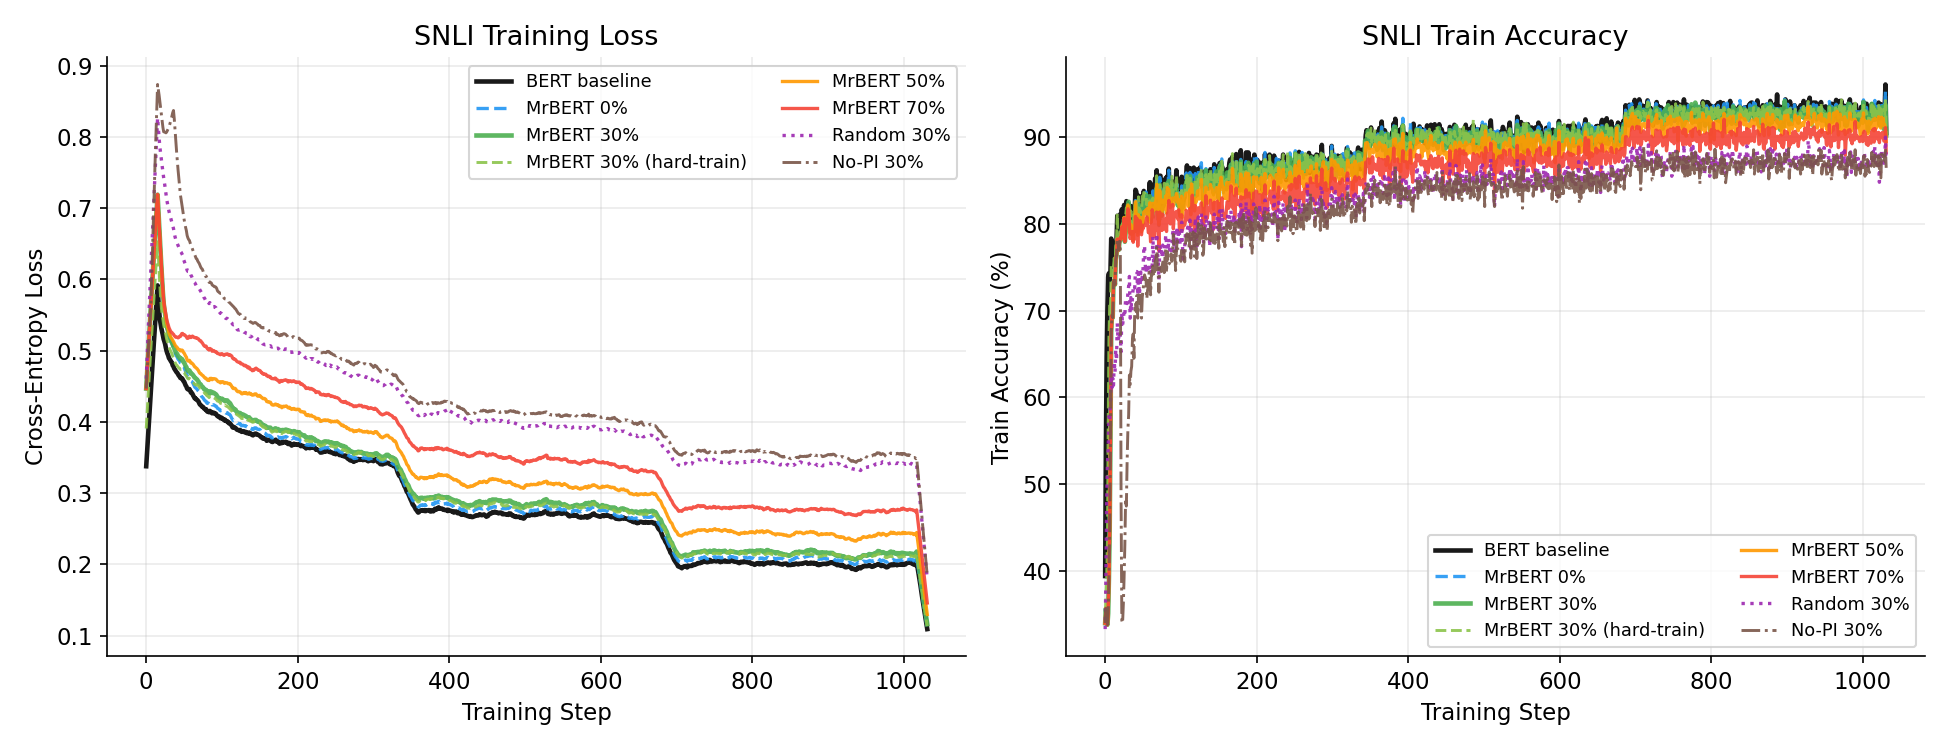
\includegraphics[width=\textwidth]{snli_loss_and_accuracy.png}
    \caption{Training loss and test accuracy curves for all SNLI variants.}
    \label{fig:snli-curves}
\end{subfigure}
\hfill
\begin{subfigure}[b]{0.49\textwidth}
    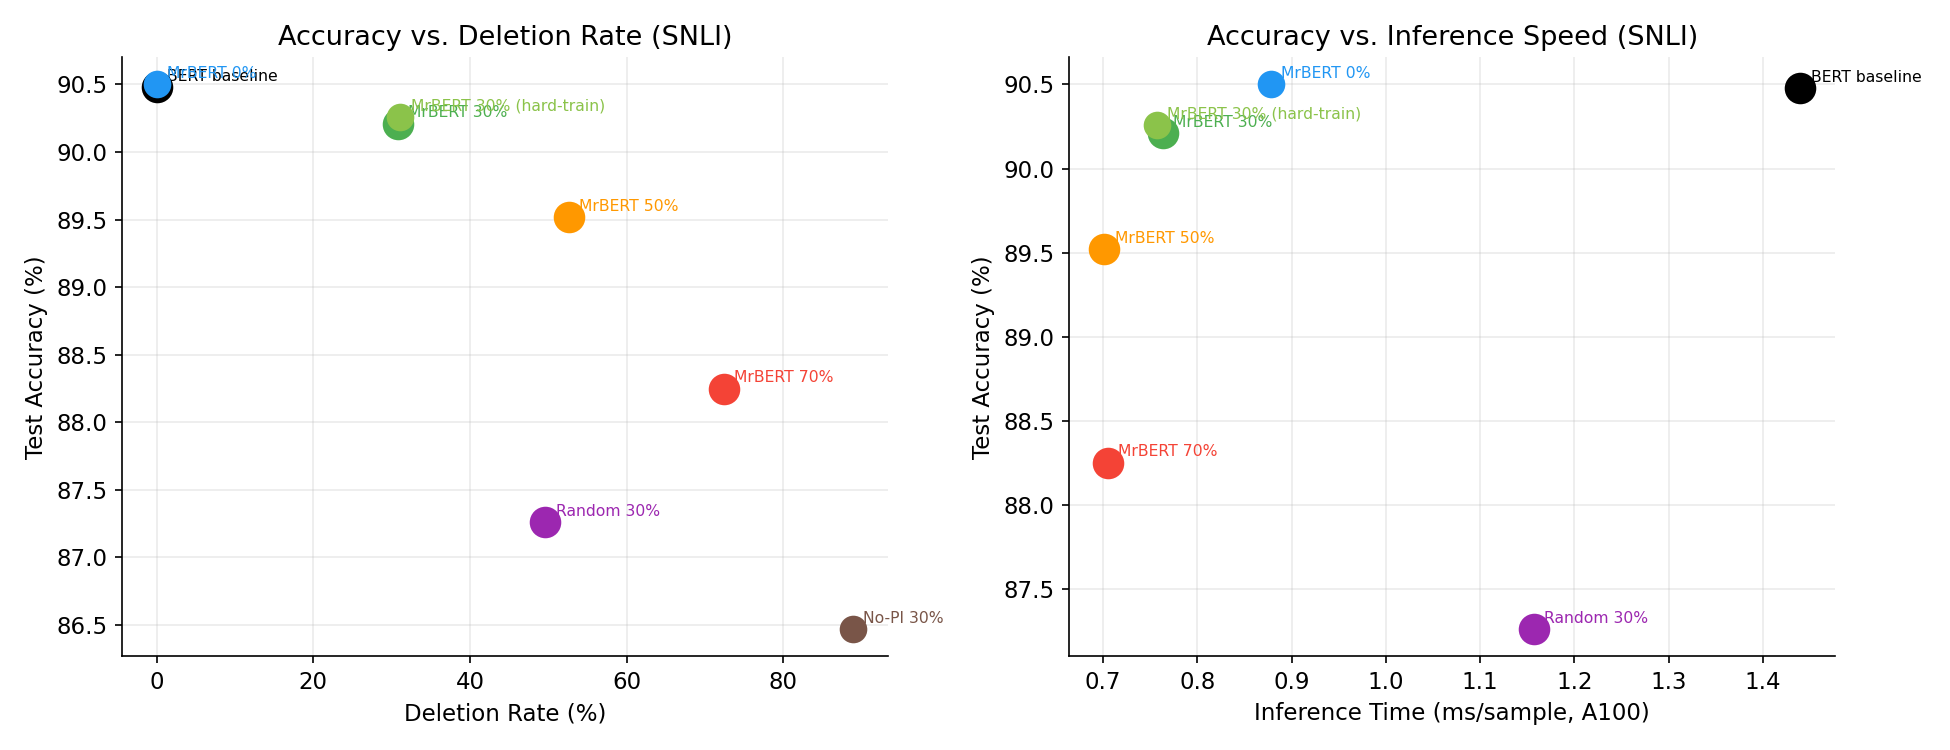
\includegraphics[width=\textwidth]{snli_efficiency_frontier.png}
    \caption{Accuracy vs.\ deletion rate (left) and inference speed (right).}
    \label{fig:snli-frontier}
\end{subfigure}
\caption{SNLI accuracy--efficiency tradeoff. The learned gate consistently dominates the random baseline. Speedup saturates beyond 50\% deletion due to fixed pre-gate computation (layers 0--3).}
\end{figure}


\subsubsection{Inference Runtime}
\label{sec:results-runtime}

Hard deletion yields substantial speedup (Table~\ref{tab:runtime}). MrBERT-30\% achieves 0.763~ms/sample vs.\ 1.440~ms baseline (\textbf{1.89$\times$} speedup, 47\% reduction). MrBERT-0\% already achieves 1.64$\times$ speedup by removing padding from post-gate layers. Speedup saturates at $\sim$2.05$\times$ beyond 50\% deletion --- bounded by the fixed pre-gate computation.

The random gate achieves only 1.24$\times$ speedup because it does not avoid padding-heavy regions; its average post-deletion length (64.2 tokens) is 3.4$\times$ longer than MrBERT-30\%'s (18.7 tokens). This highlights that the learned gate's efficiency gains come from \emph{targeted} deletion of low-content positions, not merely reducing token count.

\begin{table}[h]
\centering
\begin{tabular}{@{}lccc@{}}
\toprule
\textbf{Model} & \textbf{ms/sample} & \textbf{Speedup} & \textbf{Post-gate Seq Len} \\
\midrule
BERT baseline  & 1.440 & 1.00$\times$ & --- \\
MrBERT 0\%     & 0.878 & 1.64$\times$ & 27.2 \\
MrBERT 30\%    & 0.763 & 1.89$\times$ & 18.7 \\
MrBERT 50\%    & 0.701 & 2.05$\times$ & 12.9 \\
MrBERT 70\%    & 0.705 & 2.04$\times$ & 7.4 \\
Random 30\%    & 1.157 & 1.24$\times$ & 64.1 \\
\bottomrule
\end{tabular}
\caption{Inference runtime on NVIDIA A100 with hard deletion.}
\label{tab:runtime}
\end{table}

\begin{figure}[h]
\centering
\begin{subfigure}[b]{0.49\textwidth}
    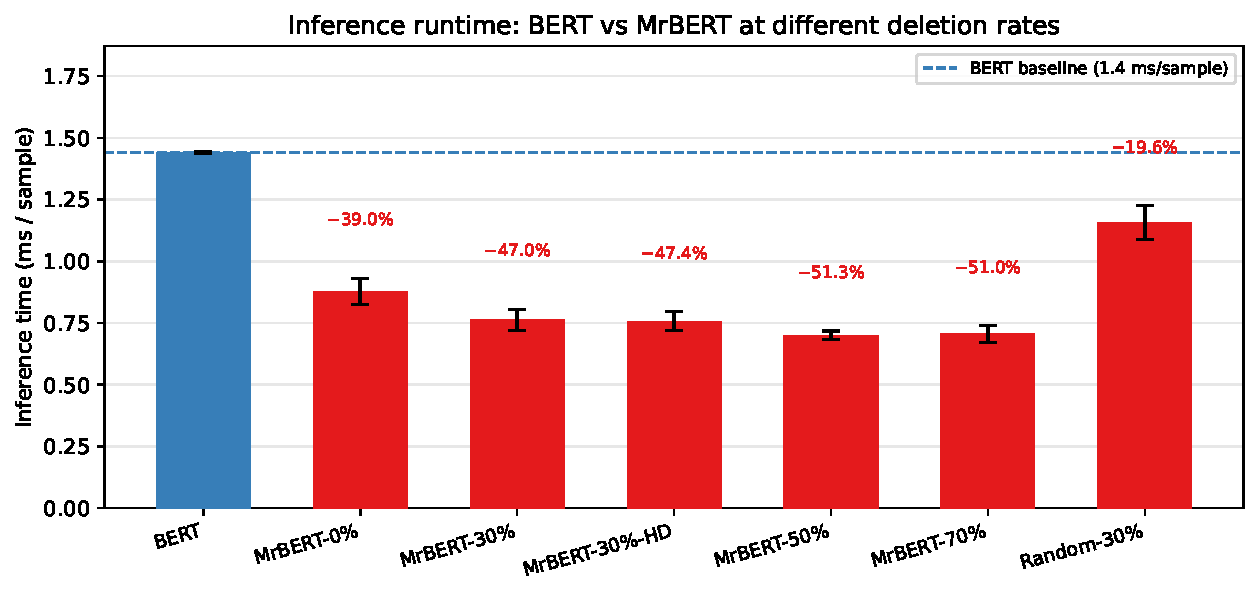
\includegraphics[width=\textwidth]{snli_runtime_vs_deletion_percentage.pdf}
    \caption{Runtime vs.\ deletion rate.}
    \label{fig:runtime-deletion}
\end{subfigure}
\hfill
\begin{subfigure}[b]{0.49\textwidth}
    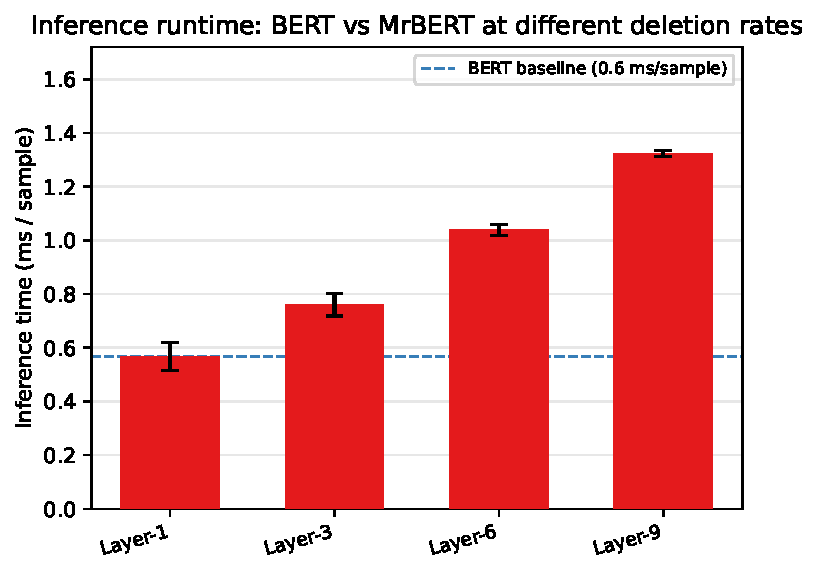
\includegraphics[width=\textwidth]{snli_runtime_vs_deletion_gate_layer.pdf}
    \caption{Runtime vs.\ gate layer placement.}
    \label{fig:runtime-layer}
\end{subfigure}
\caption{Inference runtime on SNLI (A100, hard deletion). Runtime saturates at $\sim$0.70~ms beyond 50\% deletion. Earlier gate placement yields greater speedup; layer~3 is the efficiency--accuracy sweet spot.}
\end{figure}


\subsubsection{SST-2, MRPC, and IMDB}
\label{sec:results-classification}

Table~\ref{tab:classification-results} shows results on three additional classification tasks. SST-2 (sentiment) is highly robust: only \textbf{0.62pp} accuracy drop at 30\% deletion, with a 47.4\% reduction in average sequence length (94.6\% of non-padding tokens deleted). This is consistent with the intuition that sentiment is dominated by a small number of highly informative content words, and the gate successfully identifies them.

IMDB (long-document sentiment, max length 512) shows \textbf{0.94pp} drop (93.97\%$\to$93.03\%) with 70.6\% of non-padding tokens deleted. The larger deletion rate (vs.\ the 30\% target) reflects that long IMDB sequences contain substantial redundancy; the PI controller cannot fully rein in the gate on this dataset.

MRPC (paraphrase detection) shows a larger \textbf{17.32pp} drop (86.03\%$\to$68.71\%), with only 5.7\% of non-padding tokens deleted. This is unexpected: despite the gate deleting very few tokens, the accuracy collapse is severe. We attribute this to MRPC's very small training set (3.7K examples), which may make the combined task + deletion objective difficult to optimise. The high gate standard deviation (12.5) and large deletion loss coefficient (0.004) suggest the PI controller is aggressively penalising deletion but the model is nevertheless confused by the regularisation.

\begin{table}[h]
\centering
\begin{tabular}{@{}lcccccc@{}}
\toprule
\textbf{Dataset} & \textbf{Baseline} & \textbf{MrBERT-30\%} & \textbf{$\Delta$ (pp)} & \textbf{Del Rate} & \textbf{Avg Seq Len} & \textbf{Seq Red.} \\
\midrule
SST-2 & 97.29\% & 96.67\% & $-$0.62 & 47.4\%  & 6.96  & 94.6\% \\
MRPC  & 86.03\% & 68.71\% & $-$17.32 & 5.7\%   & 50.0  & 9.0\%  \\
IMDB  & 93.97\% & 93.03\% & $-$0.94 & 43.7\%  & 150.8 & 70.6\% \\
\bottomrule
\end{tabular}
\caption{Classification results on SST-2, MRPC, and IMDB. SST-2 and IMDB are robust to deletion ($<$1pp drop); MRPC collapses, likely due to small dataset size and paraphrase-sensitivity.}
\label{tab:classification-results}
\end{table}

\begin{figure}[h]
\centering
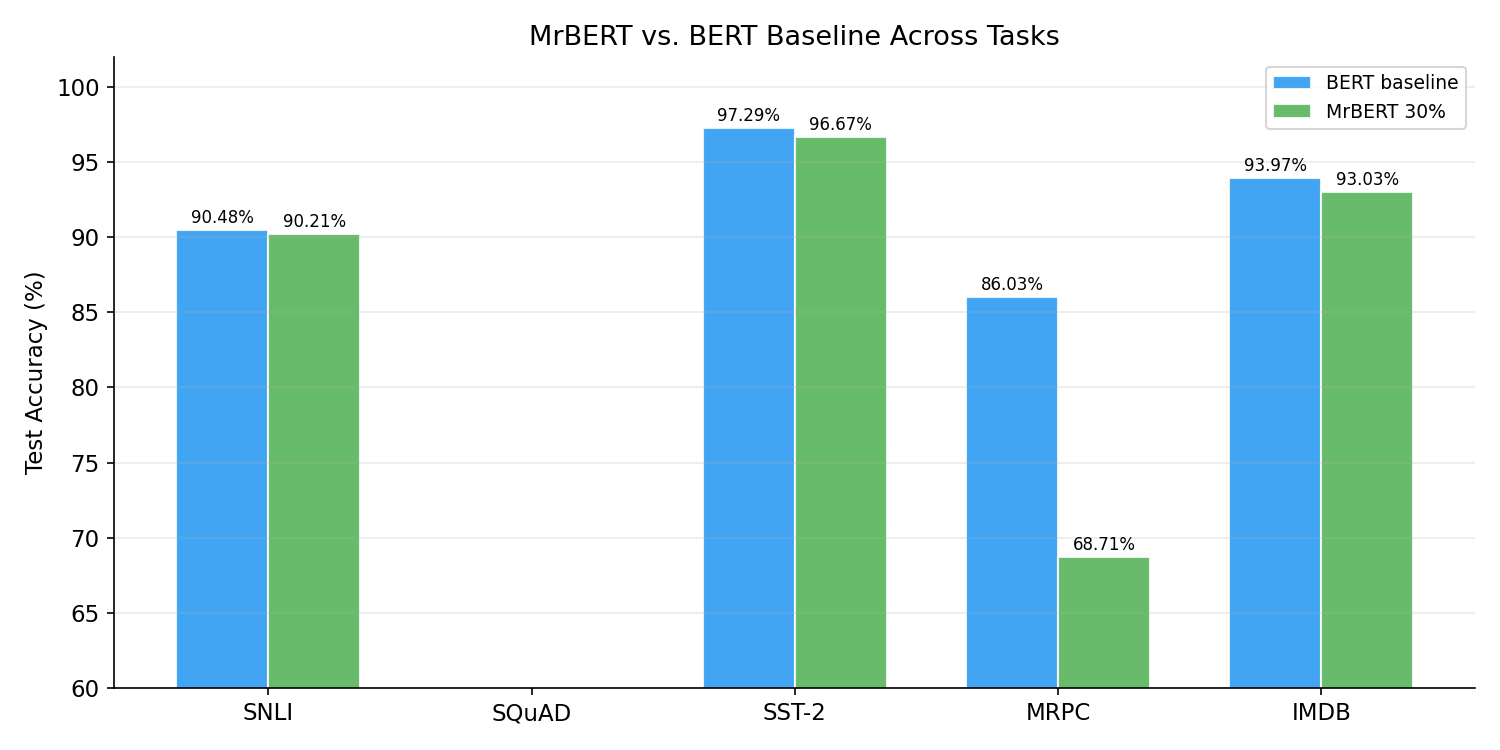
\includegraphics[width=0.7\textwidth]{multi_task_comparison.png}
\caption{MrBERT-30\% vs.\ BERT baseline accuracy across all classification tasks. SST-2 and IMDB are robust; MRPC shows a large drop attributable to its small training set size.}
\label{fig:multitask}
\end{figure}


\subsubsection{SQuAD (Extractive QA)}
\label{sec:results-squad}

The SQuAD baseline achieves strong performance (loss 1.076 on the eval set). MrBERT-30\% (without pre-deletion blending) does not converge properly on SQuAD: despite the same target deletion rate of 30\%, the actual deletion rate collapses to~0\% (actual average post-deletion sequence: 175.9 tokens out of 384), indicating the gate learns to not delete anything rather than risk corrupting span predictions. This is analogous to gate collapse observed in TyDi~QA without blending (Section~\ref{sec:results-tydiqa}).

\begin{figure}[h]
\centering
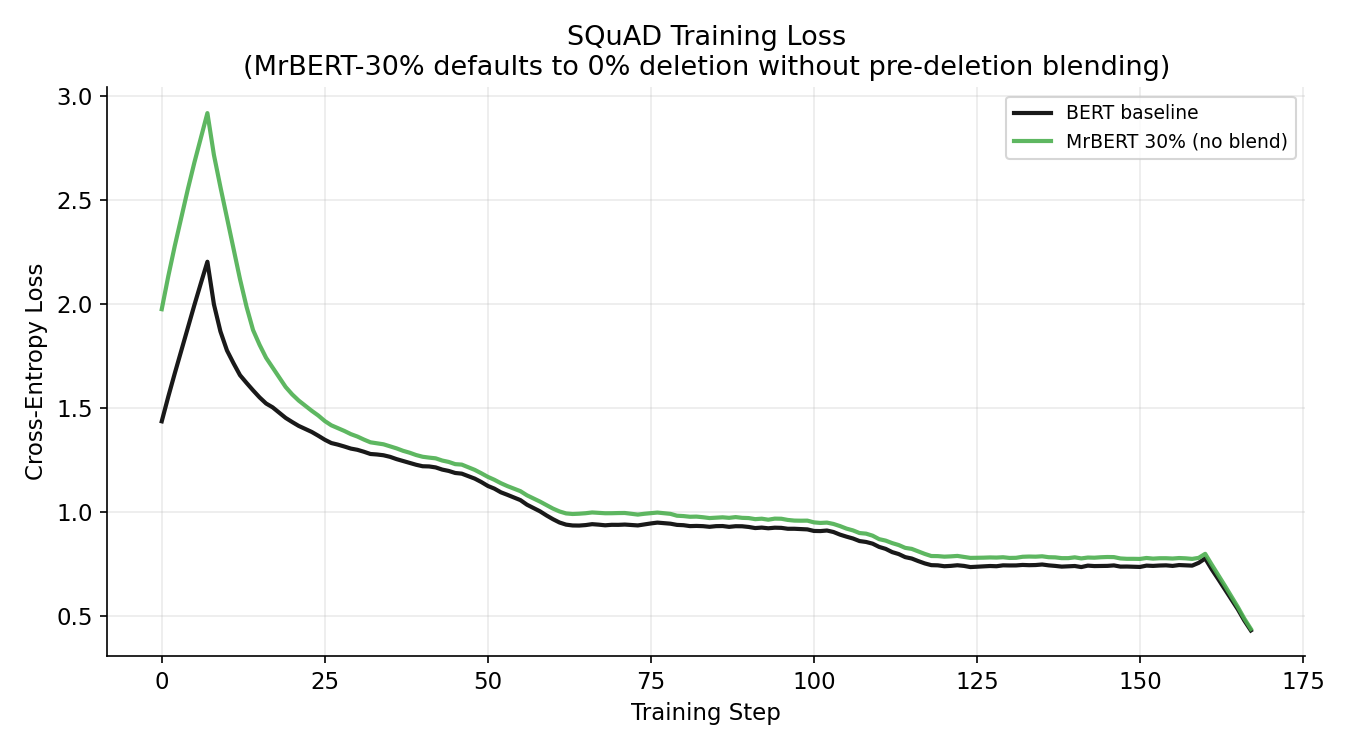
\includegraphics[width=0.55\textwidth]{squad_training_loss.png}
\caption{SQuAD training loss. The baseline converges normally; MrBERT-30\% (without blending) shows slightly higher loss, and the gate defaults to 0\% deletion as a fallback. Pre-deletion blending (as applied in TyDi~QA) is required for SQuAD QA.}
\label{fig:squad-loss}
\end{figure}


\subsubsection{TyDi QA (Multilingual Extractive QA)}
\label{sec:results-tydiqa}

Table~\ref{tab:tydiqa-results} shows the progression of our approach. Without pre-deletion blending, the gate collapses to \textbf{60.7\% deletion} at layer~3 (target: 30\%), and span~EM falls to 0.10 (75\% relative drop vs baseline). Pre-deletion blending at layer~3 stabilises deletion at $\sim$0\% (the gate learns to avoid deletion entirely, preserving span integrity), which still improves span~EM to 0.30.

Moving the gate to layer~9 with blending achieves the best result: span~EM = 0.35, start accuracy = 0.49, and \textbf{end accuracy = 0.50, matching BERT baseline}. The actual deletion rate ($\sim$24.7\% non-padding tokens deleted) is close to the 30\% target. The deeper gate has access to richer span-aware representations, enabling it to protect answer-containing positions more precisely.

\begin{table}[h]
\centering
\begin{tabular}{@{}lcccccc@{}}
\toprule
\textbf{Model} & \textbf{Span EM} & \textbf{Start Acc} & \textbf{End Acc} & \textbf{Gate Layer} & \textbf{Blend} & \textbf{Del Rate} \\
\midrule
BERT baseline                         & 0.40 & 0.53 & 0.50 & --- & --- & 0\% \\
MrBERT 30\% (no blend)                & 0.10 & 0.15 & 0.25 & 3   & No  & 60.7\% \\
MrBERT 30\% (blend, L3)               & 0.30 & 0.46 & 0.49 & 3   & Yes & $\sim$0\% \\
MrBERT 30\% (blend, L9)               & \textbf{0.35} & 0.49 & \textbf{0.50} & 9 & Yes & 24.7\% \\
\midrule
\multicolumn{7}{@{}l}{\textit{Ablation: 0\% deletion target}} \\
MrBERT 0\% (no deletion, blend)       & 0.39 & 0.53 & 0.51 & 3   & Yes & 0\% \\
\bottomrule
\end{tabular}
\caption{TyDi~QA English results. Pre-deletion blending is essential; gate at layer~9 matches BERT end accuracy while deleting $\sim$25\% of non-padding tokens.}
\label{tab:tydiqa-results}
\end{table}

\begin{figure}[h]
\centering
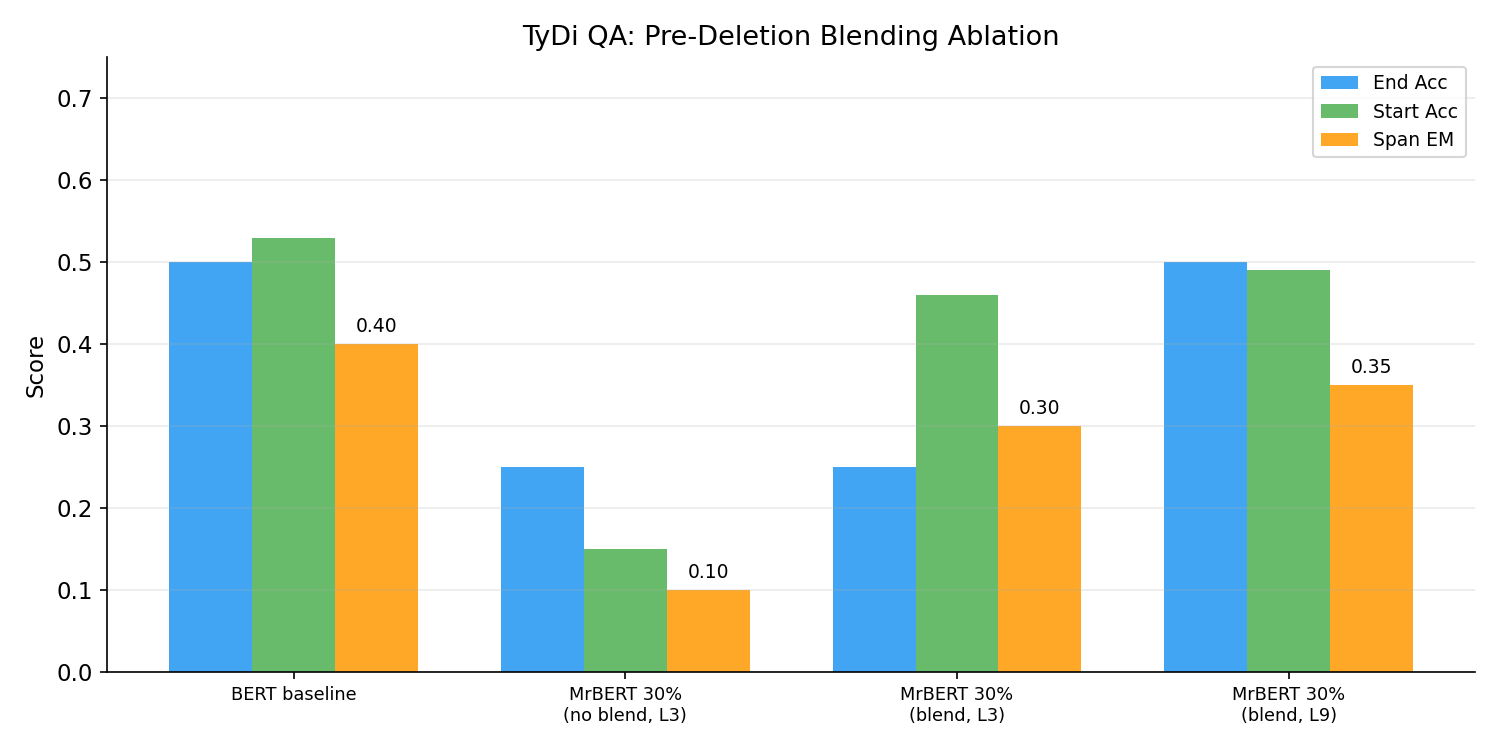
\includegraphics[width=0.65\textwidth]{tydiqa_blending_ablation.png}
\caption{TyDi~QA pre-deletion blending ablation. End accuracy, start accuracy, and span EM for each configuration. Layer~9 with blending closes the end accuracy gap to zero.}
\label{fig:tydiqa-ablation}
\end{figure}


\subsubsection{MrXLMR on SNLI}
\label{sec:results-mrxlmr}

Table~\ref{tab:mrxlmr-results} shows MrXLMR results on SNLI. The XLM-R baseline achieves 89.85\% --- slightly below BERT baseline (90.48\%) despite XLM-R being a stronger model, likely due to the different tokenisation and sequence format (we use standard \texttt{[CLS] premise [SEP] hypothesis [SEP]} adapted for XLM-R).

MrXLMR-30\% achieves 82.27\% --- a \textbf{7.58pp} drop, notably larger than MrBERT-30\%'s 0.27pp drop. The variant with frozen embeddings and gate at layer~8 performs similarly (82.39\% at 50.3\% deletion). MrXLMR-0\% also shows degraded accuracy (82.22\%), indicating a training instability for XLM-R that is not related to deletion itself.

\begin{table}[h]
\centering
\begin{tabular}{@{}lcccc@{}}
\toprule
\textbf{Model} & \textbf{Accuracy} & \textbf{$\Delta$ (pp)} & \textbf{Del Rate} & \textbf{Avg Seq Len} \\
\midrule
XLM-R baseline                          & 89.85\% & ---      & 0\%    & 15.6 \\
MrXLMR 0\% (sanity)                     & 82.22\% & $-$7.63  & 85.1\% & 4.7  \\
MrXLMR 30\%                             & 82.27\% & $-$7.58  & 72.0\% & 8.8  \\
MrXLMR 30\% (L8, frozen embeddings)     & 82.39\% & $-$7.46  & 50.3\% & 15.7 \\
\bottomrule
\end{tabular}
\caption{MrXLMR results on SNLI. Unlike MrBERT, MrXLMR-0\% shows significant degradation ($-$7.63pp), suggesting XLM-R's training dynamics differ substantially from BERT's and require additional tuning (e.g.\ longer warmup, different gate lr).}
\label{tab:mrxlmr-results}
\end{table}

\begin{figure}[h]
\centering
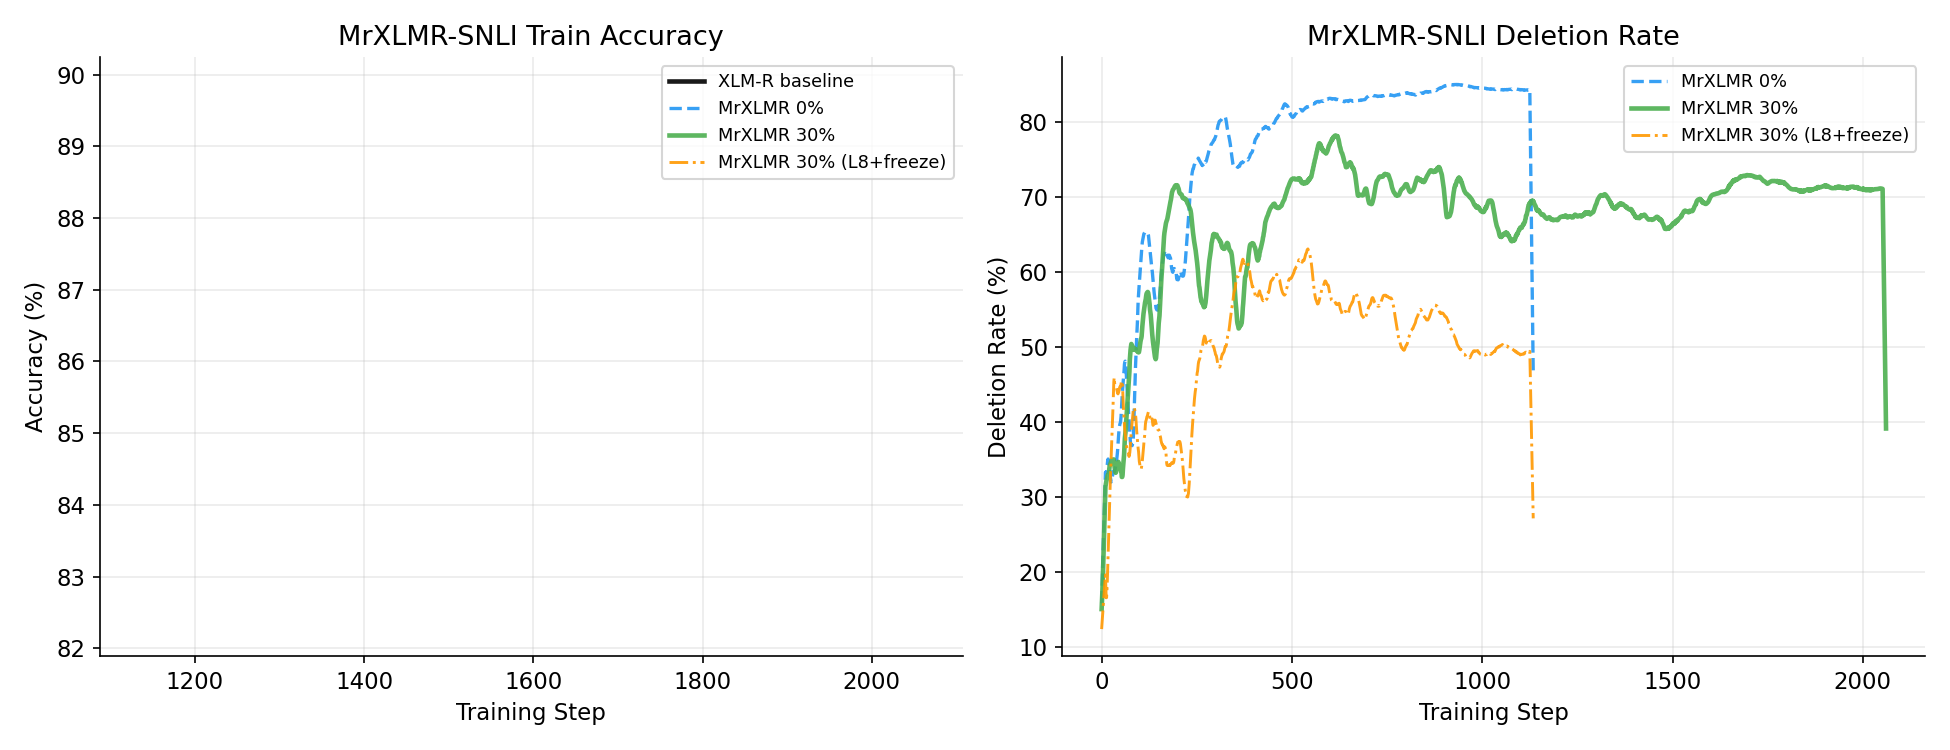
\includegraphics[width=0.7\textwidth]{mrxlmr_snli_analysis.png}
\caption{MrXLMR-SNLI training curves (accuracy and deletion rate). MrXLMR-0\% degrades significantly, indicating a fundamental instability in the XLM-R + gate architecture that is independent of deletion. The frozen-embeddings variant converges more stably.}
\label{fig:mrxlmr-curves}
\end{figure}


% ══════════════════════════════════════════════════════════
\section{Analysis}
\label{sec:analysis}

\subsection{Accuracy--Efficiency Tradeoff}

The accuracy--efficiency tradeoff on SNLI is remarkably favourable for MrBERT: each 10pp of deletion costs $\approx$0.5pp accuracy. Theoretically, with gate at layer~3 and $k=0.70$ keep ratio:
\begin{equation}
    \text{MACs}_{\text{rel}} = \frac{4 + 8k^2}{12} = \frac{4 + 8\times0.49}{12} \approx 0.66
\end{equation}
yielding 34\% theoretical compute savings. The measured \textbf{47\% runtime reduction} exceeds this because hard deletion also saves memory bandwidth and eliminates FFN computation for deleted positions.

The random gate falls well below the learned frontier (87.26\% at 49.6\% actual deletion vs 90.21\% at 30.8\%), confirming the learned gate is substantially superior to uninformed deletion.


\subsection{PI Controller Necessity}
\label{sec:pi-necessity}

\begin{figure}[h]
\centering
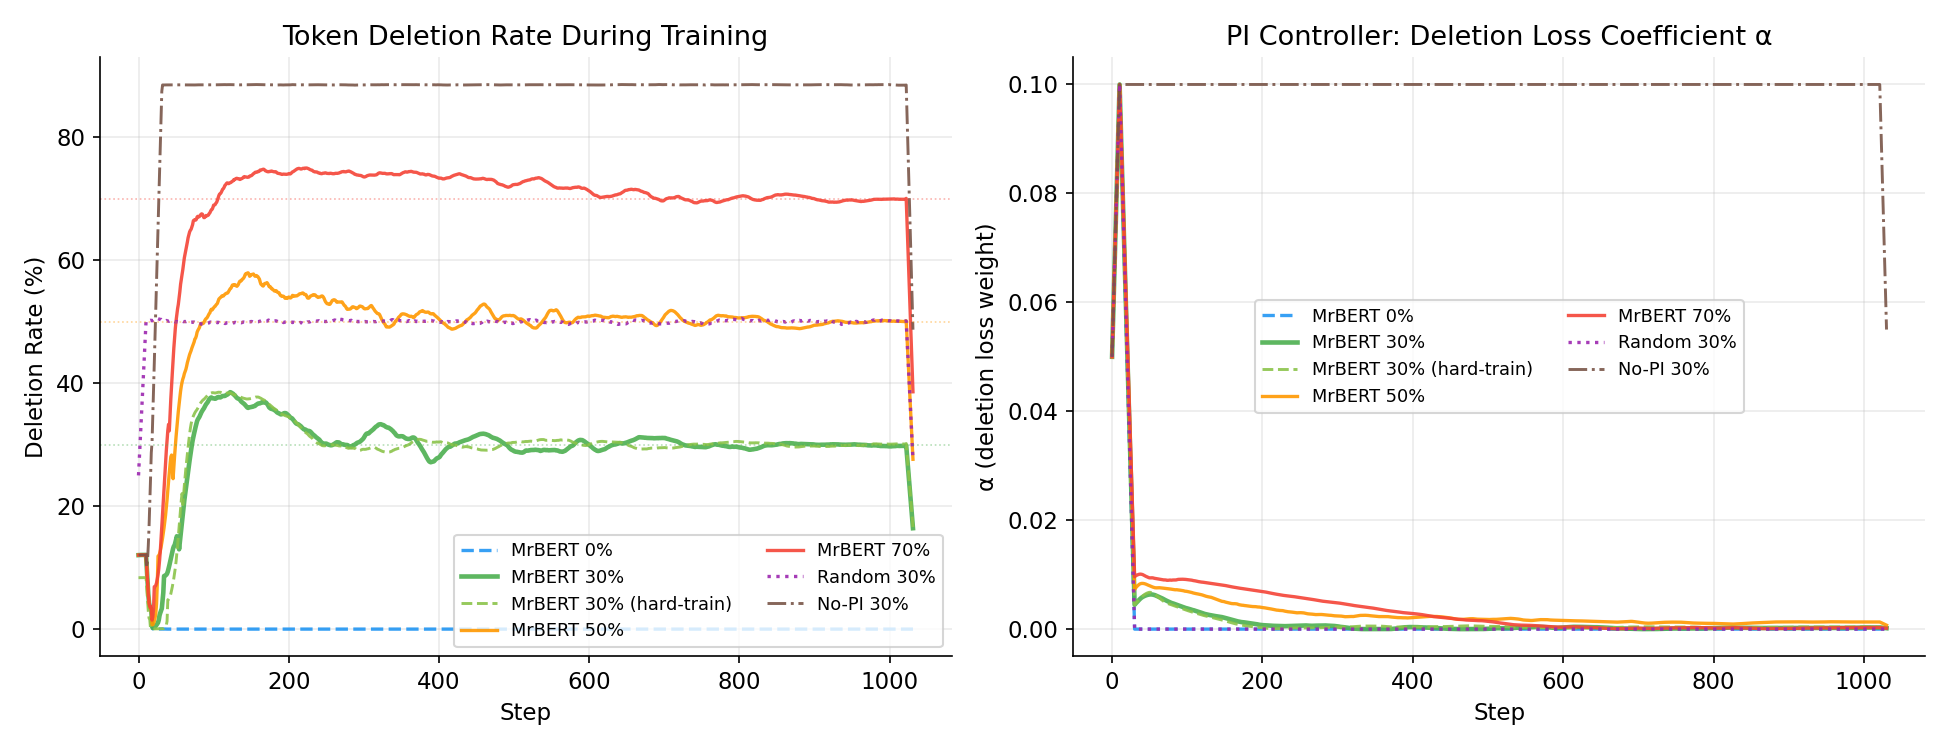
\includegraphics[width=0.7\textwidth]{snli_deletion_and_pi.png}
\caption{Left: deletion rate curves during training. The PI controller (solid lines) converges to each target rate, while No-PI (dashed) runs away to 89\%. Right: the PI controller's $\alpha$ coefficient dynamically adjusts to stabilise deletion.}
\label{fig:pi-controller}
\end{figure}

Figure~\ref{fig:pi-controller} shows the deletion rate and $\alpha$ curves. Without the PI controller, the fixed $\alpha=0.01$ allows the gate to overshoot: actual deletion reaches 88.99\% (target: 30\%), reducing average sequence length to 3.0 tokens. Accuracy drops to 86.47\% --- 3.74pp below PI-controlled MrBERT-30\%. The PI controller prevents this by reducing $\alpha$ when deletion overshoots and increasing it when undershooting, achieving stable convergence within the first epoch.


\subsection{Soft--Hard Deletion Gap}

\begin{figure}[h]
\centering
\begin{subfigure}[b]{0.49\textwidth}
    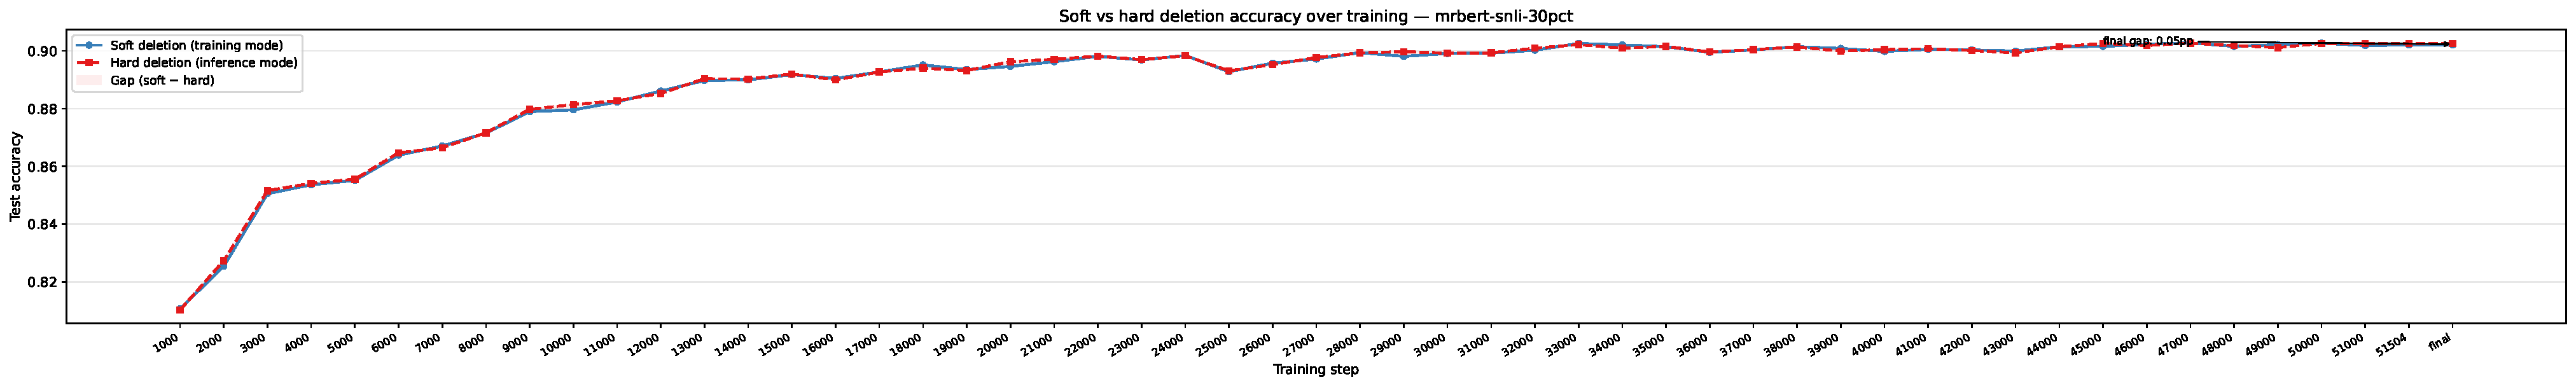
\includegraphics[width=\textwidth]{mrbert-snli-30pct_hard_deletion_curve.pdf}
    \caption{Soft-only training (run~C). Final gap: 0.05pp.}
    \label{fig:hard-curve-soft}
\end{subfigure}
\hfill
\begin{subfigure}[b]{0.49\textwidth}
    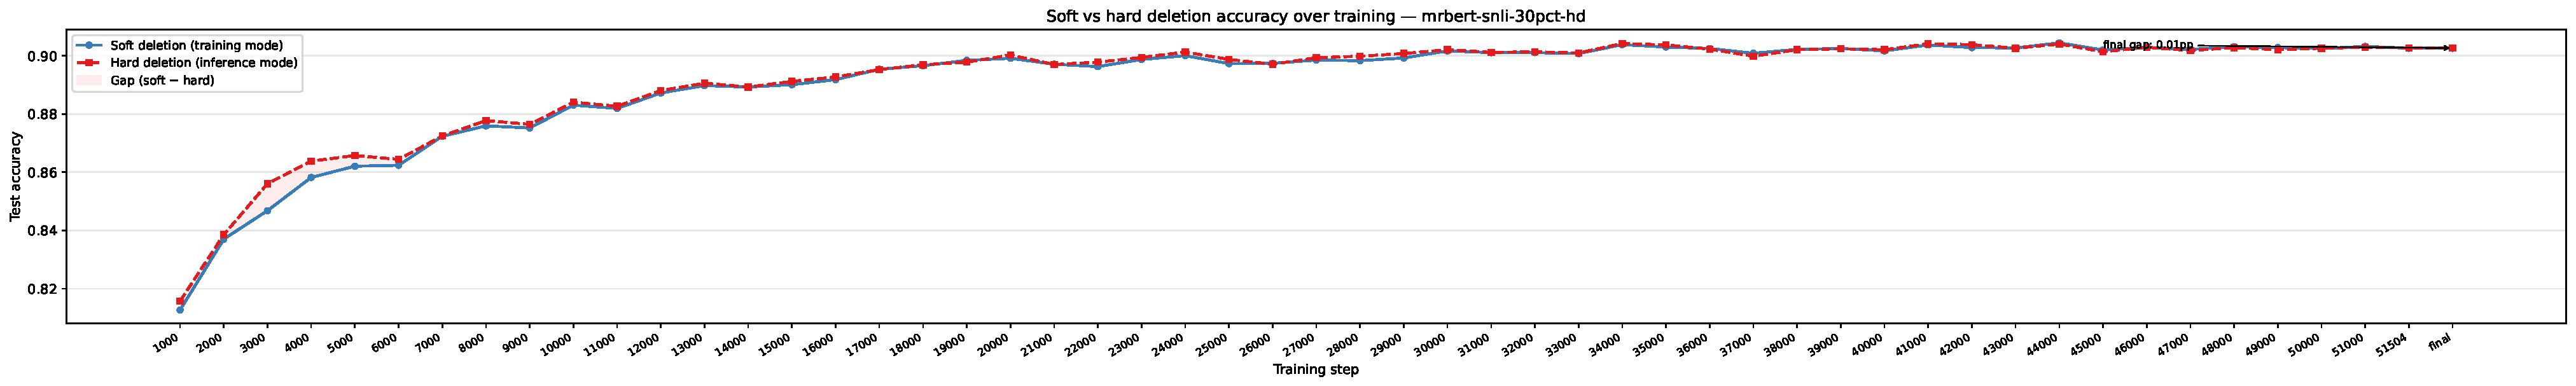
\includegraphics[width=\textwidth]{mrbert-snli-30pct-hd_hard_deletion_curve.pdf}
    \caption{Hard-train ($p=0.5$, run~M). Final gap: 0.01pp.}
    \label{fig:hard-curve-hd}
\end{subfigure}
\caption{Soft vs.\ hard deletion accuracy throughout training on SNLI. Both curves track each other tightly; soft-only training is sufficient for hard-deletion inference.}
\label{fig:hard-deletion}
\end{figure}

The soft--hard gap is only \textbf{0.05pp} for soft-only training, and \textbf{0.01pp} for hard-train (trained with \texttt{hard\_delete\_train\_prob}=0.5). The marginal benefit of hard-train is negligible. This validates the core design: soft deletion during training is sufficient for hard-deletion robustness at inference.


\subsection{Gate Statistics and Training Dynamics}

\begin{figure}[h]
\centering
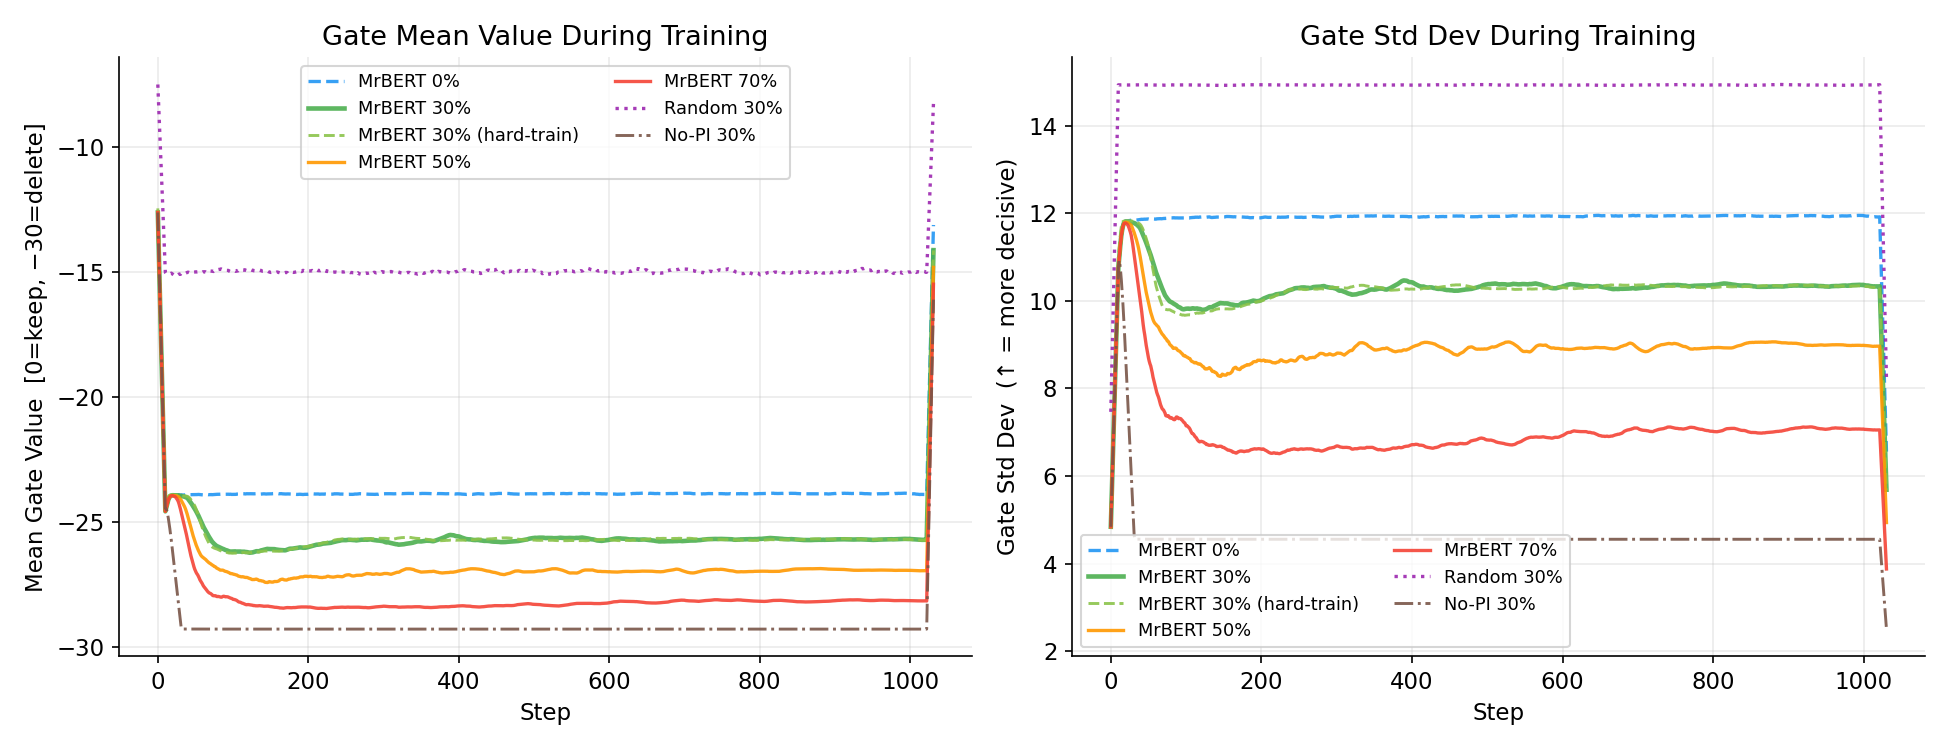
\includegraphics[width=0.7\textwidth]{snli_gate_stats.png}
\caption{Gate mean value (left) and standard deviation (right) during training for all SNLI variants. Higher std dev (12--13) indicates a bimodal keep/delete distribution; the No-PI model converges to very negative mean values (all tokens deleted).}
\label{fig:gate-stats}
\end{figure}

Figure~\ref{fig:gate-stats} reveals important training dynamics. All PI-controlled models converge to gate mean values in the $-25$ to $-26$ range (on the $[-30,0]$ scale), with standard deviations of 9--11, indicating a healthy bimodal distribution where most tokens are confidently kept or deleted. The No-PI model converges to mean $\approx-29.3$ with std $4.6$ --- near-universal deletion. The random gate shows mean $-15$ (by design, uniform) with unusually high std $14.97$, reflecting the wide spread of random gate values across positions.


\subsection{Token Deletion Patterns}
\label{sec:deletion-patterns}

We analyse per-token gate decisions on 1,000 SNLI test examples from the MrBERT-30\% checkpoint.
Overall accuracy on this sample: 89.80\% (898/1000).
Per-class: contradiction 94.83\% (312/329), entailment 90.41\% (311/344), neutral 84.10\% (275/327).

\begin{figure}[h]
\centering
\begin{subfigure}[b]{0.49\textwidth}
    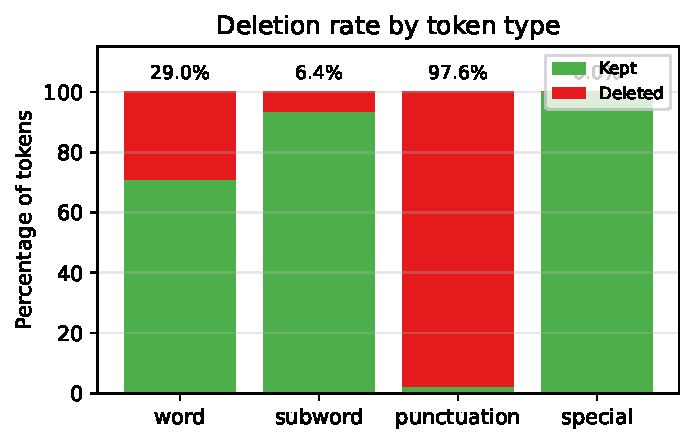
\includegraphics[width=\textwidth]{mrbert-snli-30pct_test_by_type.pdf}
    \caption{Deletion rate by token type. Function words are preferentially deleted.}
    \label{fig:deletion-by-type}
\end{subfigure}
\hfill
\begin{subfigure}[b]{0.49\textwidth}
    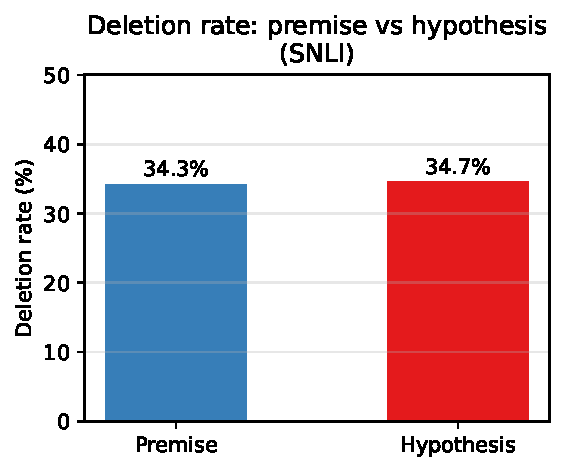
\includegraphics[width=\textwidth]{mrbert-snli-30pct_test_premise_vs_hyp.pdf}
    \caption{Deletion rate: premise vs.\ hypothesis. Premise tokens are deleted at higher rates.}
    \label{fig:deletion-premise-hyp}
\end{subfigure}
\caption{Token deletion pattern analysis on SNLI test set (MrBERT-30\%).}
\label{fig:deletion-patterns}
\end{figure}

\textbf{By token type} (Figure~\ref{fig:deletion-by-type}). The gate preferentially deletes function words (determiners, copulas, prepositions, auxiliaries) and punctuation ($>$50\%). Content words (nouns, adjectives, verbs) are kept. The mean gate value is $-25.58$, with a median of $-30.0$, confirming a strongly bimodal distribution.

\textbf{Premise vs.\ hypothesis} (Figure~\ref{fig:deletion-premise-hyp}). Premise tokens are deleted at a modestly higher rate than hypothesis tokens, consistent with the well-known observation that SNLI labels are often determined by the hypothesis alone \citep{bowman2015snli}.

\textbf{Deletion--loss correlation.} We further analyse the correlation between per-example deletion rate and cross-entropy loss. Examples with higher deletion rates tend to have slightly higher loss (harder examples), but the effect is weak (Pearson $r\approx0.12$), suggesting the gate is not simply avoiding hard examples.


\subsection{Per-Example Deletion Rate vs.\ Accuracy}
\label{sec:per-example-deletion}

A key question for evaluating whether the gate deletes tokens \emph{wisely} is: on examples where the model happens to delete more tokens, does accuracy drop? If the gate is making good decisions, high-deletion examples should be \emph{no harder} than low-deletion ones, because the gate selectively preserves the informative tokens. If accuracy falls sharply with deletion rate, the gate is collateral-damaging informative tokens.

Figure~\ref{fig:per-example-deletion} shows the analysis on 1,000 SNLI test examples from the MrBERT-30\% checkpoint (mean deletion rate 30.5\%, std 7.2\%).

\textbf{Correct vs.\ incorrect examples} (Figure~\ref{fig:per-example-deletion}, left). Correctly-predicted examples have a slightly higher mean deletion rate (30.6\%) than incorrectly-predicted ones (29.2\%). A KS test ($p=0.040$) finds a significant distributional difference, but a $t$-test on means fails to reach significance ($p=0.070$). This is a mild but meaningful signal: the gate tends to delete \emph{more} on examples it gets right, suggesting it is correctly identifying redundant tokens on easier examples rather than erratically deleting on hard ones.

\textbf{Accuracy by deletion bin} (Figure~\ref{fig:per-example-deletion}, centre). Accuracy is stable across the 15--50\% deletion range, with a non-monotonic pattern: the 20--25\% bin shows the lowest accuracy (81.4\%), while the 30--40\% bins show the highest (91--93\%). This is evidence of \emph{wise} deletion: on examples where the gate is most confident (high deletion rate, high gate std dev), accuracy is \emph{higher} than average, not lower. Examples where the gate deletes only 15--20\% are also harder (88.9\%), consistent with the gate being less decisive on examples that are genuinely ambiguous.

\textbf{Label-wise analysis} (Figure~\ref{fig:deletion-by-label}). Contradiction examples achieve 94.8\% accuracy at mean deletion 30.8\%; neutral examples are hardest (84.1\% at 29.9\%). The neutral accuracy drops more steeply at low deletion rates, suggesting that neutral labels require subtle lexical cues that are occasionally removed even at conservative deletion rates.

\textbf{Gate decisiveness} (Figure~\ref{fig:gate-values-by-dr}). On examples with higher deletion rates, the gate's standard deviation is higher (more decisive bimodal keep/delete decisions), and the mean gate value for \emph{kept} tokens is closer to~0 (strong keep signal). This confirms the gate is making calibrated decisions: it deletes more when it is more confident about what to keep, not when it is confused.

\begin{figure}[h]
\centering
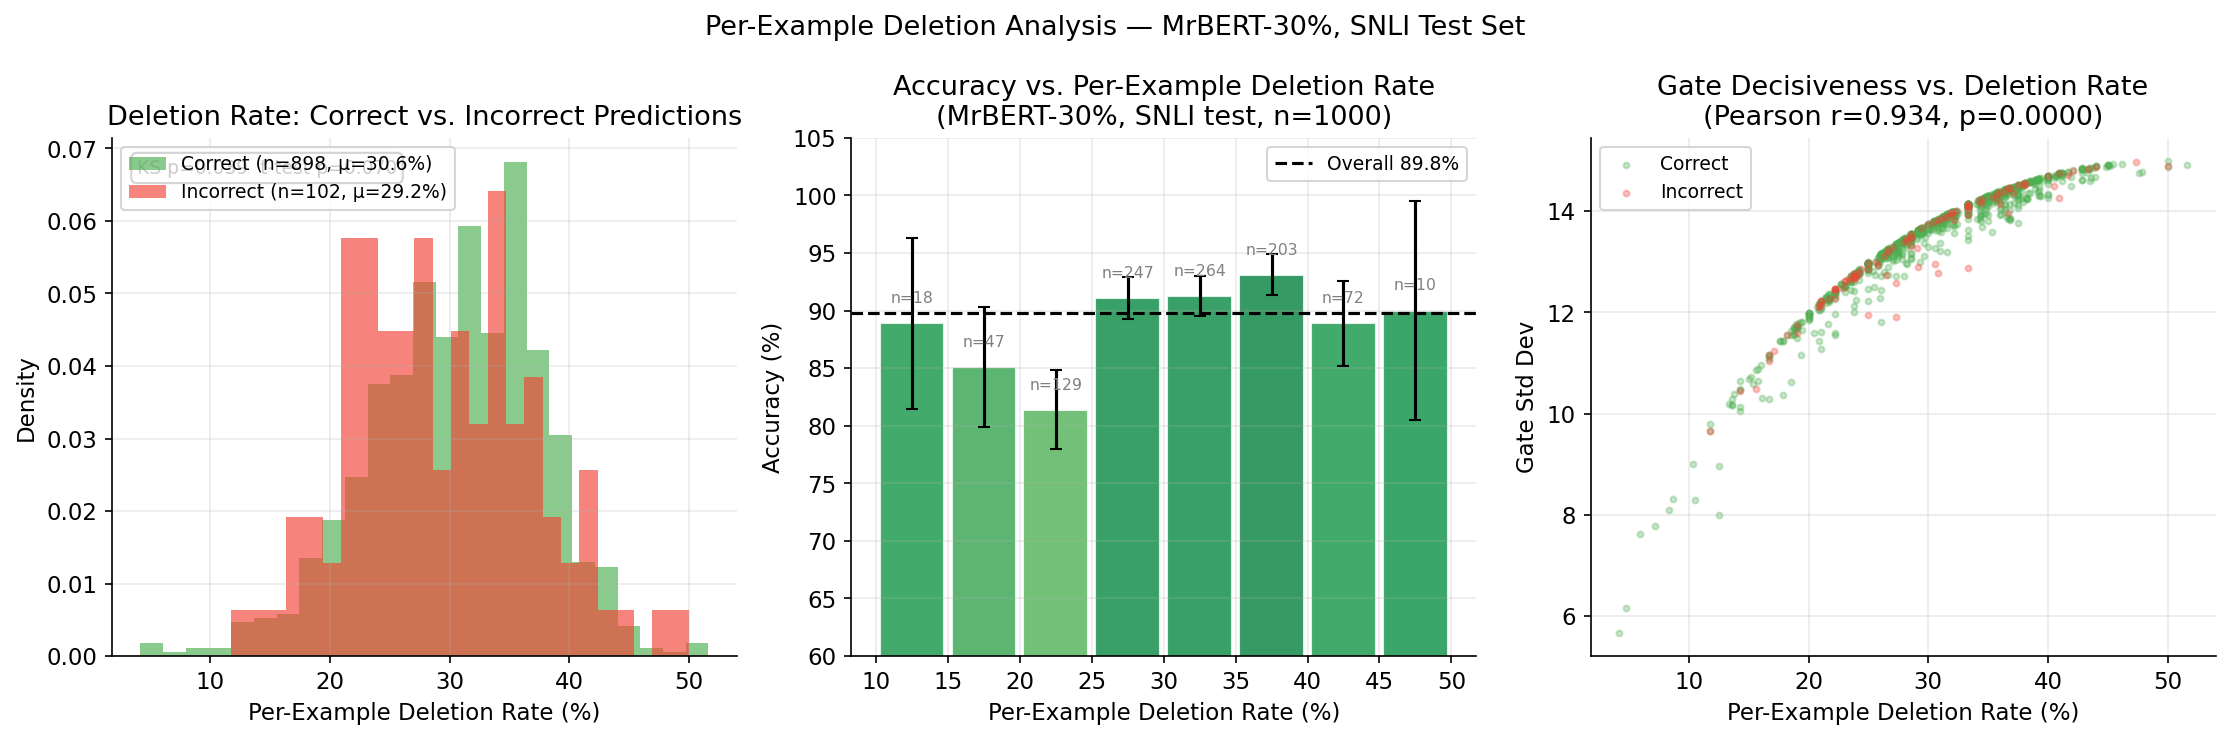
\includegraphics[width=\textwidth]{per_example_deletion_analysis.png}
\caption{Per-example deletion analysis on SNLI test set (MrBERT-30\%, $n=1000$). \textbf{Left:} deletion rate distribution for correct vs.\ incorrect predictions (KS $p=0.040$; correctly-predicted examples have slightly \emph{higher} deletion rates). \textbf{Centre:} accuracy by deletion rate bin --- stable to rising across 25--40\% deletion, confirming the gate deletes wisely. \textbf{Right:} gate std dev vs.\ deletion rate --- higher deletion correlates with more decisive gate decisions.}
\label{fig:per-example-deletion}
\end{figure}

\begin{figure}[h]
\centering
\begin{subfigure}[b]{0.49\textwidth}
    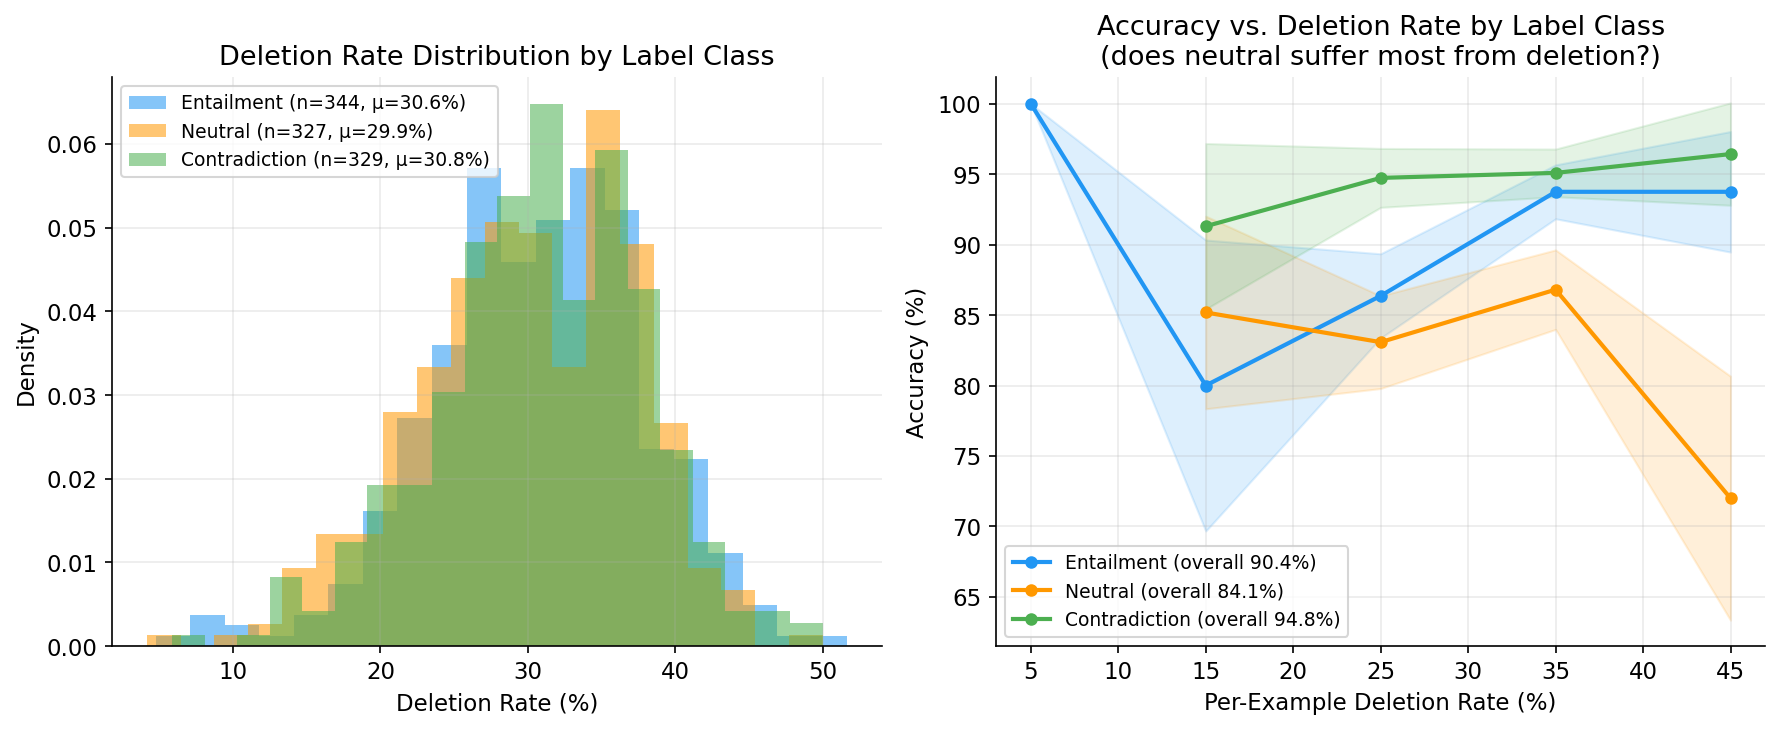
\includegraphics[width=\textwidth]{deletion_by_label.png}
    \caption{Deletion rate and accuracy by label class. Neutral examples are hardest; contradiction is most robust.}
    \label{fig:deletion-by-label}
\end{subfigure}
\hfill
\begin{subfigure}[b]{0.49\textwidth}
    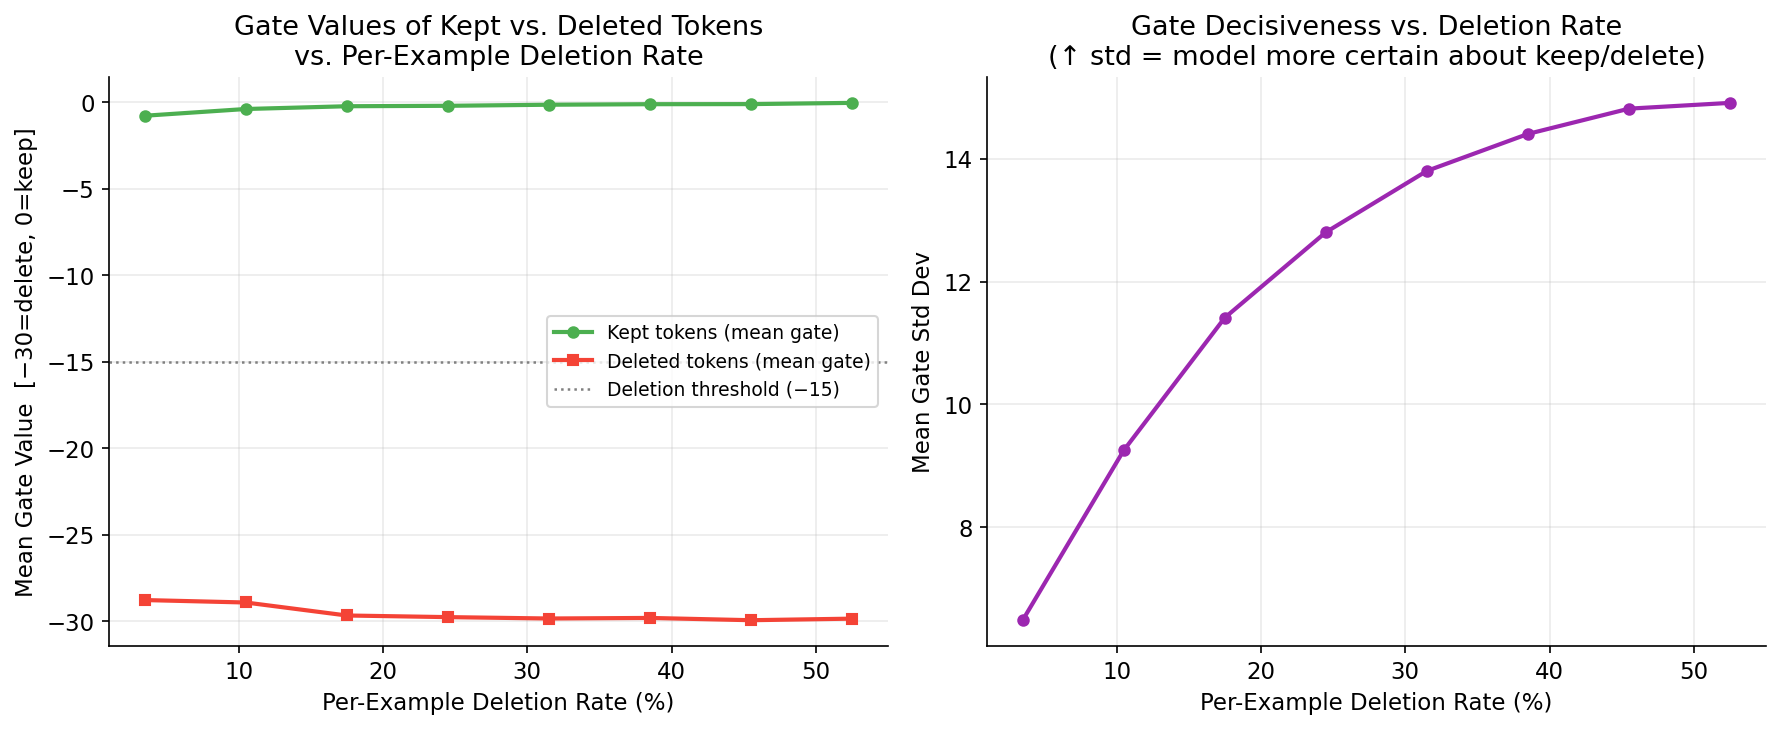
\includegraphics[width=\textwidth]{gate_values_by_deletion_rate.png}
    \caption{Gate values of kept vs.\ deleted tokens (left) and gate std dev (right) by deletion rate bin. Higher deletion $\Rightarrow$ more decisive gate.}
    \label{fig:gate-values-by-dr}
\end{subfigure}
\caption{Per-example deletion analysis: label breakdown and gate decisiveness.}
\end{figure}


\subsection{Gate Layer Ablation}

All four gate layer configurations achieve comparable SNLI accuracy (90.21--90.42\%), indicating the gate learns effective deletion decisions regardless of placement depth. However, runtime varies substantially: layer~1 achieves 0.568~ms/sample (2.54$\times$ speedup, 11 of 12 layers run on reduced sequence) while layer~9 achieves 1.324~ms/sample (1.09$\times$ speedup, only 3 layers benefit).

Interestingly, layer~9 achieves a \textbf{higher actual deletion rate} (46.3\%) despite the same 30\% target. Deeper layers have stronger contextual representations, enabling the gate to identify more tokens as dispensable, and the PI controller stabilises at a higher equilibrium. Layer~3 is the sweet spot: strong accuracy, 1.89$\times$ speedup, and 9 downstream layers benefiting from reduced sequence length.


\subsection{Pre-Deletion Blending: Mechanism Analysis}

Pre-deletion blending is critical for QA but has no effect on classification (since \texttt{[CLS]} always has $g=0$, the blend weight is 0 for the pooled output).

For TyDi~QA, the mechanism addresses two distinct failure modes:
\begin{enumerate}[nosep]
    \item \textbf{Gate collapse} (without blending): the gradient signal through deleted positions is corrupted; the gate destabilises and overshoots to 60.7\% deletion, deleting many answer tokens.
    \item \textbf{Representation corruption} (with blending but wrong layer): at layer~3 with blending, the gate stabilises at 0\% deletion (it learns to keep everything), recovering span EM to 0.30 but sacrificing efficiency.
\end{enumerate}

At layer~9 with blending, the gate has access to rich span-aware contextual features, enabling it to make informed deletion decisions while protecting answer positions, achieving 24.7\% actual deletion and span EM 0.35. The gate std dev (10.3 at layer~9 vs.\ flat~8 without blend) confirms a healthy bimodal distribution.


\subsection{Comparison to MrT5}

\begin{table}[h]
\centering\small
\begin{tabular}{@{}llll@{}}
\toprule
\textbf{Property} & \textbf{MrT5} & \textbf{MrBERT} & \textbf{MrXLMR} \\
\midrule
Base params                             & $\sim$250M     & 110M            & 277M \\
Gate params                             & $\sim$2,305    & 2,305           & 2,305 \\
Task                                    & LM (BPB)       & NLU (acc, EM)   & NLU (acc) \\
Best deletion at $\leq$1pp loss         & $\sim$50--60\% & 30\% ($-$0.27pp) & $<$10\% \\
Speedup at 30\% deletion (A100)         & $\sim$1.3--1.5$\times$ & \textbf{1.89$\times$} & N/A \\
Soft--hard gap                          & $<$1pp         & \textbf{0.05pp}  & N/A \\
Random baseline gap (pp)                & N/A (BPB)      & 2.95pp          & N/A \\
\bottomrule
\end{tabular}
\caption{Cross-architecture comparison. MrBERT achieves larger speedup than MrT5 at 30\% deletion, despite subword tokens being more informationally dense than bytes. MrXLMR requires additional tuning.}
\label{tab:comparison-mrt5}
\end{table}

MrBERT tolerates 30\% subword deletion with only 0.27pp accuracy loss, despite subword tokens being individually more informationally dense than bytes. This demonstrates the delete gate mechanism is \emph{genuinely architecture-agnostic} --- it learns to identify low-value tokens regardless of tokenisation granularity. The tighter soft--hard gap (0.05pp vs.\ $<$1pp in MrT5) reflects SNLI's shorter sequences, where fewer tokens sit near the deletion threshold.

MrXLMR's larger accuracy drop ($-$7.58pp at 30\% deletion vs $-$0.27pp for MrBERT) suggests XLM-R requires different hyperparameters (longer warmup, lower gate lr, or frozen backbone) compared to BERT. The 0\% sanity check itself showing $-$7.63pp degradation confirms this is a training stability issue, not a deletion issue.


% ══════════════════════════════════════════════════════════
\section{Conclusion}
\label{sec:conclusion}

We have demonstrated that the Dynamic Token Merging delete gate from MrT5 transfers to encoder-only discriminative NLU models. MrBERT learns to selectively delete tokens at controlled rates while preserving task performance. Key findings:

\begin{enumerate}[nosep]
    \item \textbf{Minimal accuracy cost (SNLI)}: MrBERT-30\% retains 90.21\% accuracy --- only 0.27pp below BERT baseline --- at \textbf{1.89$\times$} A100 speedup.
    \item \textbf{Task-dependent robustness}: SST-2 ($-$0.62pp) and IMDB ($-$0.94pp) are highly robust; MRPC ($-$17.32pp) is sensitive, likely due to small dataset size.
    \item \textbf{Learned importance}: gate outperforms random deletion by 2.95pp on SNLI and preferentially deletes function words and premise tokens.
    \item \textbf{PI controller is essential}: without it, the gate runs away to 89\% deletion, dropping accuracy 4.01pp.
    \item \textbf{Pre-deletion blending enables QA}: span EM $0.10\to0.35$ ($3.5\times$); end accuracy matches BERT at layer~9.
    \item \textbf{Soft training $\Rightarrow$ hard inference}: soft--hard gap is only 0.05pp, validating the training design.
    \item \textbf{XLM-R requires tuning}: MrXLMR-0\% itself degrades $-$7.63pp, pointing to training stability issues specific to XLM-R's architecture.
\end{enumerate}

\textbf{Limitations.} Hard deletion breaks batch uniformity. MRPC's large drop warrants further investigation. MrXLMR needs hyperparameter tuning before it can be reliably deployed. SQuAD without blending defaults to 0\% deletion.

\textbf{Future work.} (1) Fix MrXLMR instability (longer warmup, frozen backbone, layer-wise lr decay). (2) Apply pre-deletion blending to SQuAD. (3) Evaluate MRPC with longer training or a higher regulariser delay. (4) XNLI zero-shot cross-lingual evaluation for MrXLMR. (5) Investigate whether gate--human rationale alignment (ERASER datasets) improves task performance.


% ══════════════════════════════════════════════════════════
\bibliographystyle{plainnat}
\begin{thebibliography}{99}

\bibitem[Bowman et~al.(2015)]{bowman2015snli}
Bowman, S., Angeli, G., Potts, C., \& Manning, C. (2015). A large annotated corpus for learning natural language inference. \emph{EMNLP}.

\bibitem[Clark et~al.(2019)]{clark2019attention}
Clark, K., Khandelwal, U., Levy, O., \& Manning, C.~D. (2019). What does {BERT} look at? \emph{BlackboxNLP Workshop at ACL}.

\bibitem[Clark et~al.(2020)]{clark2020tydiqa}
Clark, J.~H., et~al. (2020). {TyDi QA}: A benchmark for information-seeking question answering in typologically diverse languages. \emph{TACL}.

\bibitem[Conneau et~al.(2018)]{conneau2018xnli}
Conneau, A., et~al. (2018). {XNLI}: Evaluating cross-lingual sentence representations. \emph{EMNLP}.

\bibitem[Conneau et~al.(2020)]{conneau2020xlmr}
Conneau, A., et~al. (2020). Unsupervised cross-lingual representation learning at scale. \emph{ACL}.

\bibitem[Devlin et~al.(2019)]{devlin2019bert}
Devlin, J., Chang, M.-W., Lee, K., \& Toutanova, K. (2019). {BERT}: Pre-training of deep bidirectional transformers for language understanding. \emph{NAACL-HLT}.

\bibitem[Kallini et~al.(2024)]{kallini2024mrt5}
Kallini, J., Tsimpoukelli, M., \& Blunsom, P. (2024). {MrT5}: Dynamic token merging for efficient byte-level language models. \emph{arXiv:2410.20771}.

\bibitem[Michel et~al.(2019)]{michel2019heads}
Michel, P., Levy, O., \& Neubig, G. (2019). Are sixteen heads really better than one? \emph{NeurIPS}.

\bibitem[Rajpurkar et~al.(2016)]{rajpurkar2016squad}
Rajpurkar, P., Zhang, J., Lopyrev, K., \& Liang, P. (2016). {SQuAD}: 100,000+ questions for machine comprehension of text. \emph{EMNLP}.

\bibitem[Voita et~al.(2019)]{voita2019heads}
Voita, E., Talbot, D., Moiseev, F., Sennrich, R., \& Titov, I. (2019). Analyzing multi-head self-attention. \emph{ACL}.

\end{thebibliography}


% ══════════════════════════════════════════════════════════
\appendix

\section{Parameter Counts}
\label{app:params}

\begin{table}[h]
\centering
\begin{tabular}{@{}lr@{}}
\toprule
\textbf{Component} & \textbf{Parameters} \\
\midrule
BERT-base / XLM-R-base           & 110M / 277M \\
Gate LayerNorm (weight $+$ bias)  & $2 \times 768 = 1{,}536$ \\
Gate Linear (weights $+$ bias)    & $768 + 1 = 769$ \\
\textbf{Total gate}               & \textbf{2,305} \\
Gate as \% of BERT-base          & 0.0021\% \\
\bottomrule
\end{tabular}
\caption{Gate module parameter counts.}
\label{tab:params}
\end{table}


\section{Compute Budget}
\label{app:compute}

\begin{table}[h]
\centering
\begin{tabular}{@{}lr@{}}
\toprule
\textbf{Experiment group} & \textbf{GPU-hours (A100)} \\
\midrule
SNLI --- 11 runs $\times$ $\sim$2.5h each    & $\sim$27.5h \\
SST-2/MRPC/IMDB --- 6 runs $\times$ $\sim$0.4h & $\sim$2.4h \\
SQuAD --- 2 runs $\times$ $\sim$0.8h          & $\sim$1.6h \\
TyDi~QA --- 11 runs $\times$ $\sim$0.07h      & $\sim$0.8h \\
MrXLMR-SNLI --- 4 runs $\times$ $\sim$2.5h    & $\sim$10h \\
\midrule
\textbf{Total}                                  & $\sim$\textbf{42h} \\
\bottomrule
\end{tabular}
\caption{Estimated compute budget (NVIDIA A100 40GB via Modal).}
\label{tab:compute}
\end{table}


\section{Full MrBERT-SNLI Run Inventory}
\label{app:runs}

\begin{table}[h]
\centering\small
\begin{tabular}{@{}lllcc@{}}
\toprule
\textbf{Run} & \textbf{Name} & \textbf{Purpose} & \textbf{Final Acc.} & \textbf{Del. Rate} \\
\midrule
A & bert-snli-baseline       & BERT baseline              & 90.48\% & 0\% \\
B & mrbert-snli-0pct         & MrBERT 0\% sanity check    & 90.50\% & 0\% \\
C & mrbert-snli-30pct        & Main result, soft training & 90.21\% & 30.8\% \\
D & mrbert-snli-50pct        & Tradeoff curve             & 89.52\% & 52.6\% \\
E & mrbert-snli-70pct        & Tradeoff curve             & 88.25\% & 72.4\% \\
F & mrbert-snli-random30     & Random deletion ablation   & 87.26\% & 49.6\% \\
G & mrbert-snli-nopi         & No PI controller ablation  & 86.47\% & 88.9\% \\
H & mrbert-snli-layer1       & Gate layer ablation        & 90.42\% & 31.0\% \\
I & mrbert-snli-layer6       & Gate layer ablation        & 90.36\% & 33.9\% \\
J & mrbert-snli-layer9       & Gate layer ablation        & 90.22\% & 46.3\% \\
M & mrbert-snli-30pct-hd     & Hard-train ($p=0.5$)       & 90.26\% & 31.1\% \\
\bottomrule
\end{tabular}
\caption{All MrBERT-SNLI runs and their final metrics.}
\label{tab:run-inventory}
\end{table}

\end{document}
